\documentclass{scrartcl}
\usepackage[utf8]{inputenc}
\usepackage[ngermanb]{babel}
\usepackage{graphicx}
\usepackage{amssymb}
\usepackage{amsmath}
\usepackage{wrapfig}
\usepackage{gensymb}
\usepackage{cite}
\usepackage{float}
\usepackage{url}
\usepackage{lscape}
\usepackage[onehalfspacing]{setspace}
\usepackage{helvet}
\usepackage{tocloft}
\usepackage{color}
\renewcommand{\familydefault}{\sfdefault}

\title{Simulation dynamischer Vorgänge im elektrischen Netz mit PSS Sincal und PSS Netomac}
\author{Felix Annen}



\begin{document}

\begin{titlepage}



\maketitle
\thispagestyle{empty}
\newpage
	\subsection*{Eidesstattliche Erklärung}
	\glqq Ich Versichere, dass ich diese Studienarbeit selbstständig und nur unter Verwendung der angegebenen Quellen und Hilfsmittel angefertigt und die benutzen Quellen als solche kenntlich gemacht habe. Die Arbeit hat in gleicher oder ähnlicher Form noch keiner Prüfungsbehörde vorgelegen\grqq \\ \\ \\
	Bielefeld, den \today


\end{titlepage}


	\pagenumbering{Roman}
	\setcounter{page}{1}
	\tableofcontents
	\newpage
	\listoffigures
	\phantomsection
	\addcontentsline{toc}{section}{Abbildungsverzeichnis}
	
	\listoftables
	\phantomsection
	\addcontentsline{toc}{section}{Tabellenverzeichnis}
	
	\newpage
	\section*{Abkürzungsverzeichnis}
	\phantomsection
	\addcontentsline{toc}{section}{Abkürzungsverzeichnis}
	\begin{tabular}{lll}
	ANSI & & American National Standards Institute \\ \\
	ASCII & & American Standard Code for Information Interchange \\ \\
	AWE & & Automatische Wiedereinschaltung \\ \\
	COMTRADE & & Common format for Transient Data Exchange for power systems \\ \\
	ESB & & Ersatzschaltbild \\ \\
	IEC & & International Electrotechnical Commission \\ \\
	KU & & Kurzunterbrechung \\ \\
	NOSPE & & Niederohmige Sternpunkterdung\\ \\
	RESPE & & Resonanzsternpunkterdung\\ \\
	VDE & & Verband der Elektrotechnik, Elektronik und Informationstechnik \\ \\
	
	\end{tabular}
	
	\newpage
	\setcounter{page}{1}
	\pagenumbering{arabic}
\begin{onehalfspace}

\section{Einleitung}
In Zeiten der Energiewende wird das Themengebiet der Zuverlässigkeit der elektrischen Netze immer bedeutender. Um Fehler und andere Vorgänge in Netzen zu verstehen, reicht es daher nicht, ausschließlich, auch die zu Grunde liegenden dynamischen Vorgänge müssen dazu betrachtet werden.

Als praxisnahes Beispiel sei hier die Aufzeichnung von Störungen in Umspannanlagen und deren Analyse genannt. Versagt der Schutz mutmaßlich, kann hinterher der gesamte Störungsvorgang duch die Aufzeichnung der Momentanwerte analysiert und im Labor nachgestellt werden. So lässt sich die eventuell unerwartete Störungsursache ermitteln und Schutzkonzepte anpassen.

\subsection{Problemstellung}
Der Bereich der elektrischen Netze wurde in der Lehre an der Fachhochschule Bielefeld in den letzten Jahren vernachlässigt. So gibt es derzeit zu den meisten Modulen in diesem Bereich keine Laborpraktika, was die gesamte Thematik zur reinen Theorie ohne jeden Praxisbezug macht. Gerade eine Fachhochschule, die sich selbst praxisorientiert nennt, sollte hier mehr bieten. Im Modul \glqq Elektrische Netze\grqq{} im Studiengang Regenerative Energien wurden bereits erste Praktika eingeführt. So müssen die Studierenden im ersten Praktikum ein Netz mit Hilfe der Software PSS Sincal aufbauen, im zweiten an diesem Lastflussberechnungen durchführen und im dritten Kurzschlüsse in diesem berechnen. Sincal bietet allerdings keine Möglichkeiten zur Darstellung der dynamischen Vorgänge von Kurzschlüssen, was zum Verständnis der Vorgänge bei Kurzschlüssen allerdings unerlässlich ist. Daher wird derzeit die Betrachtung des dynamischen Verlaufs der Kurzschlussströme komplett weggelassen, was sich in Zukunft aber ändern soll.

\subsection{Aktueller Stand}
Vor dem breiten Einzug von Computern in die Lehre wurden Drehstromnetzmodelle eingesetzt, an denen das Verhalten von Netzen anschaulich dargestellt werden konnte. In diesen waren angetriebene Synchronmaschinen als Generator, Transformatoren, Leitungen und Lasten enthalten. Das Verhalten des Netzes konnte direkt mit einem Oszilloskop oder Leistungsmessern gemessen werden. Auch die FH Bielefeld besaß ein solches Modell, welches allerdings nicht mehr existiert.

Mit dem Einzug von modernen Computern in die Hochschulen kamen auch Netzberechnungsprogramme in die Lehre.

Im Laborpraktikum der Universität Magdeburg wird als Software Netdraw zur Netzmodellierung, Laku zur Lastflussberechnung und Netomac zur Berechnung dynamischer Vorgänge eingesetzt. Dies wird so seit den 1990er Jahren praktiziert. Mit Netdraw lassen sich elektrische Netze modellieren und direkt aus der Benutzeroberfläche Berechnungen mit Laku oder NETOMAC durchführen.
Heutzutage ist Netdraw nicht mehr zeitgemäß und da an der FH Bielefeld schon länger die Netzplanungssoftware Sincal eingesetzt wird, soll mit dieser das Netz modelliert werden. Aus Sincal heraus lassen sich direkt Lastfluss- und Kurzschlussberechnungen durchführen, allerdings lässt sich nicht deren dynamischer Verlauf darstellen. Zur Berechnung von dynamischen Vorgängen existiert eine Exportfunktion nach NETOMAC, welche dazu genutzt werden soll. NETOMAC und Sincal werden von Siemens vertrieben und sind in Deutschland zum Quasistandard von Netzplanungen und Netzanalysen geworden. Sie werden von vielen Netzbetreibern, aber auch von Anlagenbetreibern, verwendet. Mit NETOMAC lassen sich nicht nur dynamische Vorgänge bei Kurzschlüssen darstellen, sondern auch Flicker und stationäre Lastflüsse, sowie elektromechanische Phänomene berechnen.
 
\subsection{Zielsetzung}
Auf Basis des Praktikumversuches \glqq Praktikum Elektrische Netze - Teil 2 Kurzschlußberechnungen\grqq{} der Otto-von-Guerike-Universität Magdeburg, auf dem auch die Laborpraktika der FH Bielefeld basieren, soll der dritte Laborversuch nun überarbeitet werden. Die Studierenden sollen dabei insbesondere die dynamischen Kurzschlussstromverläufe analysieren. Unterschiedliche Fehlerarten und unterschiedliche Fehlerorte sollen anhand des Verlaufs erkannt werden können. Dazu soll die Software NETOMAC genutzt werden, um die dynamischen Verläufe darzustellen.

Dementsprechend müssen die Praktikumsunterlagen überarbeitet werden. Am Ende soll eine Praktikumsanleitung für Studierende, eine Anleitung für Mitarbeiter und eine Musterlösung ausgearbeitet werden.

NETOMAC bietet sich in diesem Fall an, weil das Programm bereits auf allen Rechnern installiert ist, auf denen auch Sincal installiert ist. Lizenzen sind daher bereits vorhanden. Desweiteren bietet Sincal eine Exportfunktion für das NETOMAC-Dateiformat an.

Die möglichst komfortable Verbindung dieser beiden Programme wird das Hauptziel dieser Bachelorarbeit sein.

Eine weitere interessante Möglichkeit zur Visualisierung von Kurzschlüssen stellt der Export der Berechnungsergebnisse von NETOMAC in das COMTRADE-Format dar. Liegt das Ergebnis als Comtrade-Datei vor, kann der Kurzschlussstromverlauf über das vorhandene Prüfgerät der Firma Kocos ausgegeben werden, sodass z.B. das Auslösen eines Schutzgerätes beobachtet werden kann.

\section{Grundlagen}


\subsection{Fehlerarten in elektrischen Netzen}
Als Fehler bezeichnet man eine Abweichung vom ungestörten Betriebszustand eines Netzes. Der bekannteste Fehler ist der Kurzschluss, bei dem mindestens zwei Potentialpunkte niederohmig miteinander verbunden sind und ein wesentlich größerer Strom als der Nennstrom fließt. Diese hohen Ströme verusachen einen Spannungseinbruch an der Fehlerstelle und, bei entsprechender Zeit, Beschädigungen an Betriebsmitteln. In Freileitungsnetzen entstehen Fehler meistens durch Bäume und Blitzeinschläge, in Kabelnetzen meistens durch mechanische Beschädigungen, z.B. durch Bauarbeiten \cite[S. 57]{Pistora2013}. Gespeist werden diese Kurzschlussströme vor allem durch Synchrongeneratoren, in kleinerem Umfang auch durch Asynchrongeneratoren. Synchronmotoren können im ersten Moment wie Synchrongeneratoren betrachtet werden, das selbe gilt für Asynchrongeneratoren und Asynchronmaschinen. Kategorisiert werden können Kurzschlüsse einmal durch die Anzahl und die Verbindungen der am Kurzschluss beteiligten Pole und durch die elektrische Entfernung zu den speisenden Generatoren. Bei ersteren unterscheidet man zwischen:

\begin{itemize}
\item Dreipoliger Kurzschluss
\item Zweipoliger Kurzschluss ohne Erdberührung
\item Zweipoliger Kurzschluss mit Erdberührung
\item Einpoliger Erdkurzschluss
\item Doppelerdschluss
\end{itemize}

Eine Besonderheit in Netzen der Mittel- und Hochspannung bis 110kV ist, dass diese oftmals gelöscht betrieben werden. Das heißt, dass einige Transformatorsternpunkte mit einer Erdschlusslöschspule geerdet sind, die parallel zur Leitungskapazität wirkt. Der Fehlerstrom eines einpoligen Fehlers wird durch die Kompensation wesentlich geringer, sodass die Chance steigt, dass sich der dazugehörige Lichtbogen von selbst löscht. Der Erdkurzschluss wird zu einem Erdschluss. (Quelle)

Das zweite Unterscheidungsmerkmal ist, ob der Fehler \glqq generatornah\grqq{} oder \glqq generatorfern\grqq{} auftritt. Dazu werden die Teilkurzschlussströme der einzelnen Zweige betrachtet, zu denen die Generatoren beitragen. Übersteigt mindestens einer dieser Teilkurzschlussströme, die durch einen Generatoren fließen, den doppelt Wert des Nennstromes des Generators, so gilt der Kurzschluss als generatornah \cite[S. 56]{Schlabbach2003}. Das Kriterium \glqq generatornah oder generatorfern\grqq{} ist also ein Merkmal für die Größe der Netzimpedanz zwischen Generatoren und Fehlerstelle. \\
%Die nachfolgenden Abschnitte beziehen sich auf symmetrische dreipolige Kurzschlüsse. Auf den einpoligen Fehler wird später eingegangen.

\subsection{Dreipoliger Kurzschluss}
Bei der Berechnung der Kurzschlussströme unterscheidet man zwischen verschiedenen Kurzschlussgrößen. Gemeinsam haben sie alle, dass sie aus dem Anfangskurzschlusswechselstrom $I_k''$ abgeleitet werden. %Die folgenden Abschnitte beziehen sich auf den generatornahen symmetrischen dreipoligen Kurzschluss.
Die Berechnung der Kurzschlussströme ist in VDE 0102 beschrieben.

\subsubsection{Anfangskurzschlusswechselstrom}
Der Anfangskurzschlusswechselstrom ist laut VDE 0102 der \glqq Effektivwert zum Zeitpunkt des Kurzschlussbeginns\grqq{} und wird wie folgt berechnet:

\begin{equation}
I_k'' = \frac{c \cdot U_n}{\sqrt{3} \cdot Z_k}
\end{equation}

Dieser steht für den subtransienten Anteil des Kurzschlussstromes, der während der ersten Halbwellen auftritt. $Z_k$ steht dabei für die Impedanz der Kurzschlussbahn und setzt sich aus der Generatorreaktanz $X_d''$, Generatorresistanz, sowie Netzreaktanz und -resistanz zusammen. Da in der Praxis die Reaktanzen wesentlich größer sind als die Resistanzen, können die Resistanzen für Überschlagsrechnungen vernachlässigt werden.

\subsubsection{Transienter Kurzschlusswechselstrom}
Nach dem Abklingen des subtransienten Anteils fließt der transiente Anteil des Kurzschlussstromes. Seinen Effektivwert berechnet sich wie folgt:

\begin{equation}
I_k' = \frac{ c \cdot U_n}{\sqrt{3} \cdot X_d'}
\end{equation}

Diese Gleichung gilt für den generatornahen Kurzschluss. Für den generatorfernen Kurzschluss kann vereinfacht $I_k' = I_k''$ angenommen werden.

\subsubsection{Stoßkurzschlussstrom}
Der Stoßkurzschlussstrom $i_p$ ist der Strom mit der höchsten Amplitude, der bei einem Kurzschluss auftritt. Dieser setzt sich aus einem Gleichstromglied und einem Wechselstromglied zusammen. Die Höhe des Stoßkurzschlussstromes hängt vom Einschaltwinkel $\psi$ und dem Netzimpedanzwinkel $\varphi_k$ ab. \\
Mathematisch lässt sich der Stoßkurzschlussstrom aus der Gleichung des zeitlichen Verlaufs herleiten \cite[S. 20]{Roeper1964}: \\

\begin{equation}
i_{(t)} = \frac{\sqrt{2} \cdot E}{Z} \cdot sin(\omega \cdot t + \psi - \varphi) + I_g \cdot e^{-t/\tau} 
\hspace{2pt} mit \hspace{2pt} I_g = \frac{\sqrt{2} \cdot E}{Z} \cdot sin( \psi -  \varphi) \hspace{2pt} und \hspace{2pt} \tau = \frac{L}{R}
\end{equation}

%(S.20 Kurzschlussstr. in Dreh…)\\
Daraus wird ersichtlich, dass der zeitliche Verlauf aus einem Wechselstromanteil und einem abklingenden Gleichstromanteil besteht. Um jetzt den Spitzenwert zu finden, muss diese Gleichung nach der Zeit t abgeleitet werden. Danach wird $i = 0$ gesetzt und nach t umgestellt. Daraus erhält man den Zeitpunkt des Spitzenwertes, welcher bei einem Einschaltwinkel von $\psi = 0$ am größten ist. Der Zeitpunkt ist nicht exakt $\omega t = \pi/2 + \varphi$, der Unterschied ist aber so gering, dass er vernachlässigt werden kann. Mit diesen Angaben läst sich nun der Strom zum Zeitpunkt $\omega t = 2/\pi + \varphi$ berechnen, welcher dem Stoßkurzschlussstrom entspricht.\\
In der Praxis wird ein Stroßfaktor $\kappa$ verwendet, was hinreichend genau ist und die Rechnung vereinfacht.
Der Stoßkurzschlussstrom berechnet sich dann aus dem Spitzenwert des Anfangskurzschlusswechselstromes multipliziert mit dem Stoßfaktor. Dieser liegt zwischen 1,0 und 2,0 und hängt vom R/X-Verhältnis des Netzes ab \cite[S. 246]{Funk1962}.
% und ist beim Einschaltwinkel $\psi = 0$, also im Spannungsnulldurchgang, am größten (Der Kurz. S. 245).
Da der Einschaltwinkel zufällig ist, muss bei der Planung immer der größte Stoßkurzschlussstrom berechnet werden, also $\psi = 0$. Dies ist in der Formel mit dem Stoßfaktor $\kappa$ bereits berücksichtigt: \\

\begin{equation}
i_p = \kappa \cdot \sqrt{2} \cdot I_k'' \hspace{5pt} mit \hspace{2pt} \kappa = 1,02 + 0,98 \cdot e^{-3 \frac{R}{X}}
\end{equation}

Die Höhe des Stoßkurzschlussstromes legt die mechanische Beanspruchung einer Anlage fest, auf die diese ausgelegt werden muss. Außerdem bestimmt er das Einschaltvermögen der Leistungsschalter \cite[S. 519]{Oeding2011}. \\

\subsubsection{Dauerkurzschlussstrom}
Der Dauerkurzschlussstrom $I_k$ beschreibt den Effektivwert des Stromes, der nach dem Abklingen aller Ausgleichsvorgänge fließt. Beim generatornahen Kurzschluss ist dieser kleiner als der Anfangskurzschlusswechselstrom $I_k''$. Er berechnet sich wie folgt:

\begin{equation}
I_k = \frac{c \cdot U_n}{\sqrt{3} \cdot X_d}
\end{equation}

 Beim generatorfernen Kurzschluss kann $I_k = I_k''$ angenommen werden. Die Ausgleichsvorgänge haben in der Realität nur einen geringen Einfluss und werden vernachlässigt.

\subsubsection{Ausschaltwechselstrom}
Der Ausschaltwechselstrom $I_b$ beschreibt den Strom, der beim Ausschaltvorgang über einen Schalter fließt und bestimmt das Schaltvermögen. Da in der Regel die Ausgleichsvorgänge noch nicht abgeschlossen sind, fließen in die Berechnung von $I_b$ die Zeit und die  subtransiente und transiente Zeitkonstante mit ein:

\begin{equation}
I_b = (I_k'' - I_k') \cdot e ^{-t/T_d''} +  (I_k' - I_k) \cdot e ^{-t/T_d'} + I_k
\end{equation}
In der Praxis wird auch hier vereinfacht. Statt aufwendig zu rechnen, wird der Anfangskurzschlusswechselstrom $I_k''$ mit einem Faktor $\mu$ multipliziert, der abhängig von der Zeit und vom Strom durch den Generator ist. Damit reduziert sich die Formel auf:

\begin{equation}
I_b =  \mu \cdot I_k''
\end{equation}

Sind die benötigten Daten laut VDE 0102 Abs. 4.5.2.1 für den Faktor $\mu$ nicht bekannt, so beträgt dieser 1. Bei generatorfernen Kurzschlüssen ist $I_b = I_k''$.
%Ia == alt Ib == neu

%Ip Bedeutung?\\
%Ik \\
%Ik' \\
%Ik'' \\
%Ith \\

\subsubsection{Spannungsfaktor c}
Da bei der händischen Berechnung der Kurzschlusswechselströme Leitungskapazitäten vernachlässigt werden und die Betriebsspannung in der Regel über der Nennspannung liegt, werden diese Faktoren mit einem Spannungsfaktor c kompensiert. Zur Berechnung der größten Kurzschlussströme beträgt er bei Hoch- und Mittelspannungsnetzen 1,1, in Niederspannungsnetzen 1,05. Sollen die kleinsten auftretenden Kurzschlussströme berechnet werden, beträgt c 1,0 in Hoch- und Mittelspannungsnetzen und 0,95 in Niederspannungsnetzen \cite[S. 537]{Oeding2011}.

\subsubsection{Dynamischer Verlauf des Kurzschlussstroms}
Der Verlauf eines Kurzschlussstromes kann aufgeteilt werden in einen Daueranteil, einen transienten Anteil und einen subtransienten Anteil. Diese ergeben überlagert den in Abbildung \ref{kss-verlauf-nah} dargestellten Verlauf.

	\begin{figure}[H]
	\centering
	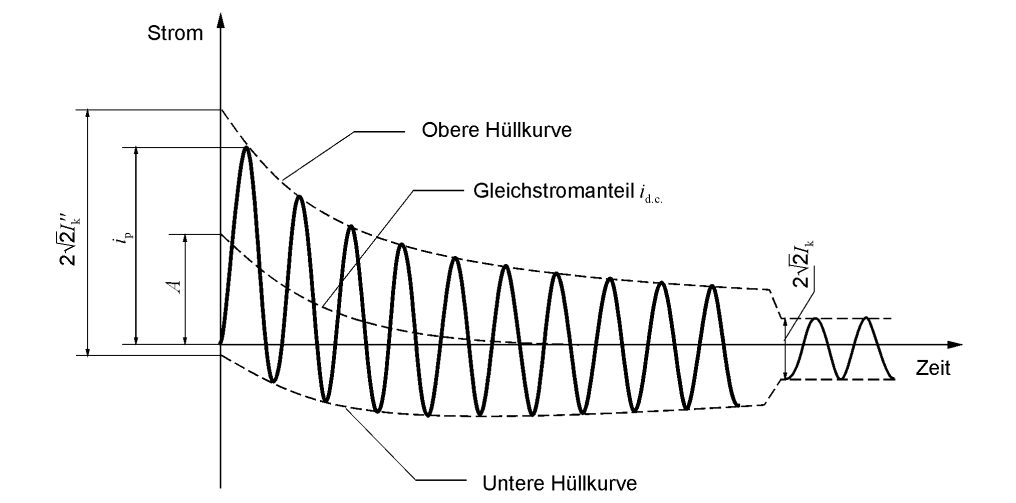
\includegraphics[scale=0.5]{img/generatornah.png}
	\caption{Verlauf des generatornahen Kurzschlussstroms}
	\label{kss-verlauf-nah}
	\end{figure}

Beim Eintritt des generatornahen Kurzschlusses wird als erstes der subtransiente Anteil sichtbar. Er klingt bereits nach ein einigen Halbwellen exponentiell mit der Zeitkonstanten $T_d''$ ab und geht in den transienten Kurzschlussstrom über, welcher wesentlich langsamer abklingt. Überlagert wird der Kurzschlussstrom noch durch einen Gleichstromanteil. Dieser kommt dadurch zustande, dass durch die überwiegend induktive Kurzschlussreaktanz der Strom bei Kurzschlusseintritt nicht \glqq springen\grqq{} kann. Aus diesem Grund wird ein Ausgleichsstrom $i_g$ erzwungen, welcher mit der Gleichstromzeitkonstanten $T_g$ abklingt. Die Höhe des Gleichstromgliedes ist abhängig vom Einschaltwinkel, also vom Einschaltzeitpunkt des Kurzschlusses, $\psi$ und ist bei $\psi = 0$ am größten.
%\\- Gleichstromglied \\
\begin{equation}
i_k(t) = \sqrt{2} \cdot [(I_k'' - I_k') \cdot e^{-t/T_d''} + (I_k' - I_k) \cdot e^{-t/T_d'} + I_k] \cdot sin(\omega t + \psi - \varphi_k) + \sqrt{2} \cdot I_k'' \cdot e^{-t/T_g} \cdot sin( \varphi_k - \psi)  \\
\end{equation}


Vernachlässigt man die Resistanzen, ersetzt die Ströme und setzt $\psi = 0$, so gelangt man zu folgender Formel für den zeitlichen Verlauf:

\begin{equation}
i_k(t) = \sqrt{2} \frac{U_n}{\sqrt{3}} [(\frac{1}{X_d''} - \frac{1}{X_d'}) e^{-t/T_d''} + (\frac{1}{X_d'} - \frac{1}{X_d}) e^{-t/T_d'} + \frac{1}{X_d}] \cdot cos(\omega t) + \sqrt{2} \frac{U_n}{\sqrt{3} X_d''} e^{-t/T_g}
\end{equation}

Aus dieser Formel werden die drei überlagerten Anteile des Kurzschlussstromes deutlich. Auf die einzelnen Reaktanzen und Zeitkonstanten wird später genauer eingegangen. \\

Für den generatorfernen Kurzschluss gilt ähnliches. Da hier die Netzimpedanz allerdings einen wesentlich höheren Einfluss hat als beim generatorfernen Kurzschluss, kann noch weiter vereinfacht werden. Es wird, wie bereits beschrieben, $I_k'' = I_k' = I_k$ angenommen. Daraus ergibt sich nun folgende Formel:

\begin{equation}
i_k(t) = \sqrt{2} \cdot I_k'' \cdot sin(\omega t + \psi - \varphi) + \sqrt{2} \cdot I_k'' \cdot e^{-t/T_g} \cdot sin(\varphi - \psi)
\end{equation}

An dem Verlauf, der in Abbildung \ref{kss-verlauf-fern} dargestellt ist, erkennt man, dass der Kurzschlussstrom, insbesondere der Gleichanteil, wesentlich schneller abklingt als der generatornahe Kurzschluss. Die Zeitkonstanten $T_d''$ und $T_d'$ entfallen, es bleibt nur die Gleichstromzeitkonstante $T_g$.

	\begin{figure}[H]
	\centering
	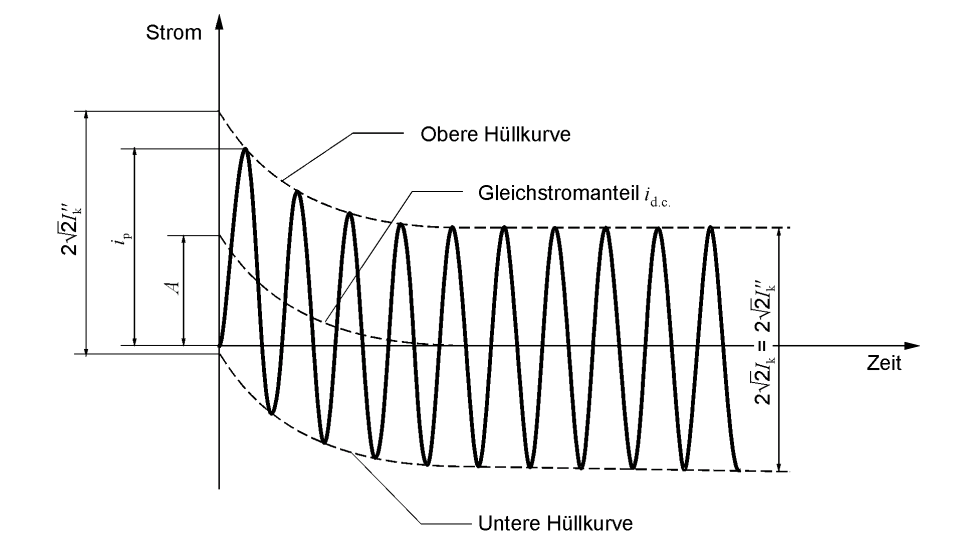
\includegraphics[scale=0.5]{img/generatorfern.png}
	\caption{Verlauf des generatorfernen Kurzschlussstroms}
	\label{kss-verlauf-fern}
	\end{figure}
	
\subsection{Einpoliger Kurzschluss}
Einpolige Fehler mit Erdberührung sind die am häufigsten auftretenden Fehler in elektrischen Netzen ab einer Nennspannung von 110kV \cite[S. 64]{Schlabbach2002}. Sie entstehen beispielsweise durch herabfallende Äste oder durchhängende Vogelnester. Üblicherweise werden Netze bis 110kV kompensiert betrieben. Dabei wird der kapazitive Anteil des Stromes an der Fehlerstelle durch eine Petersenspule kompensiert, die zwischen dem Sternpunkt des Transformators und dem Erdreich angeschlossen wird. Kleinere Mittelspannungsnetze, beispielsweise in Industrieanlagen, werden auch mit isoliertem Sternpunkt betrieben. Netze mit höheren Spannungen werden starr geerdet. Man nennt dies \glqq Niederohmige Sternpunkterdung\grqq{} (NOSPE). Der Erdschlussstrom wird dann zu einem Erdkurzschlussstrom. Grundsätzlich wird unter folgenden Sternpunktbehandlungen unterschieden:

\begin{itemize}
\item Niederohmige Sternpunkterdung (NOSPE): Abbildung \ref{sternpunktbehandlung}a
\item Resonanzsternpunkterdung (RESPE): Abbildung \ref{sternpunktbehandlung}c
\item Isolierter Sternpunkt: Abbildung \ref{sternpunktbehandlung}b
\item Strombegrenzende Erdung: Abbildung \ref{sternpunktbehandlung}d
\end{itemize}
% Dadurch, dass der Fehlerstrom nicht kompensiert wird, löst der Schutz aus und der fehlerbehaftete Netzabschnitt wird sofort abgeschaltet.
%\\ Verlauf einpoliger Fehler?

	\begin{figure}[H]
	\centering
	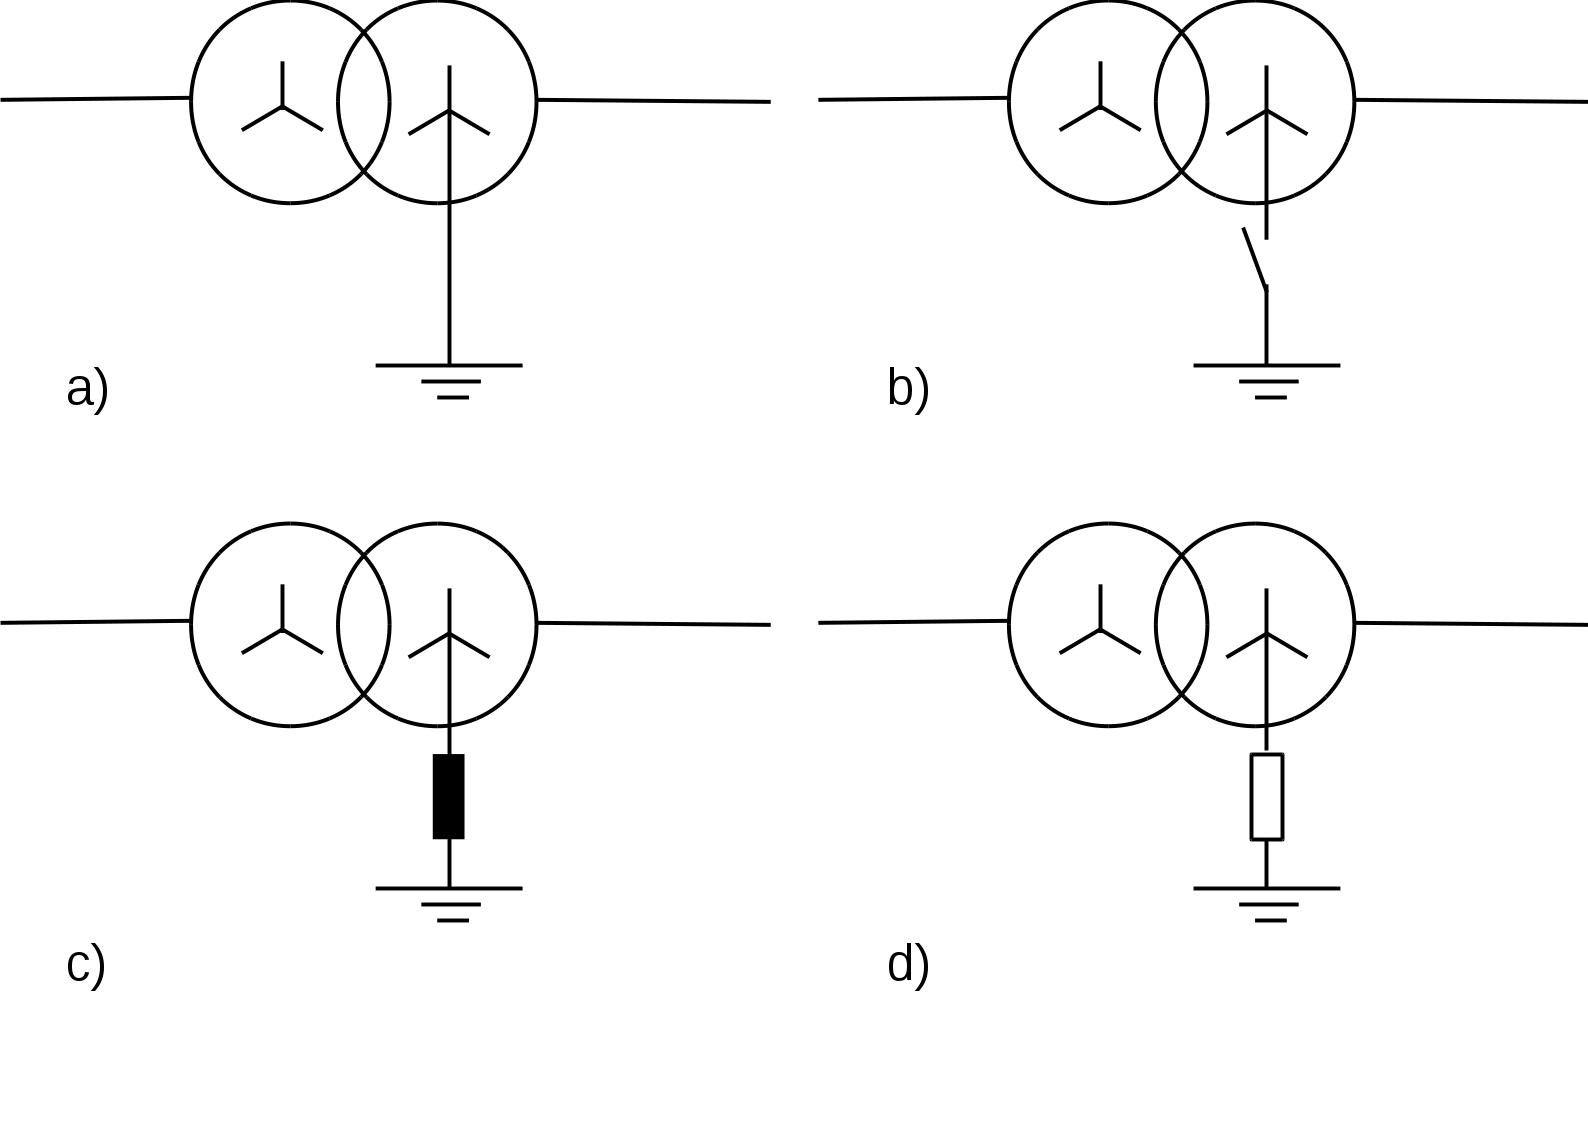
\includegraphics[scale=0.3]{img/sternpunktbehandlung.png}
	\caption{Sternpunktbehandlungen}
	\label{sternpunktbehandlung}
	\end{figure}

\subsubsection{Darstellung in symmetrischen Komponenten}
Da einpolige Fehler unsymmetrisch sind, müssen zur Berechnung symmetrische Komponenten hergezogen werden. In symmetrischen Komponenten sind einpolige Fehler eine Reihenschaltung aus Mit-, Gegen- und Nullsystem: \\

	\begin{figure}[H]
	\centering
	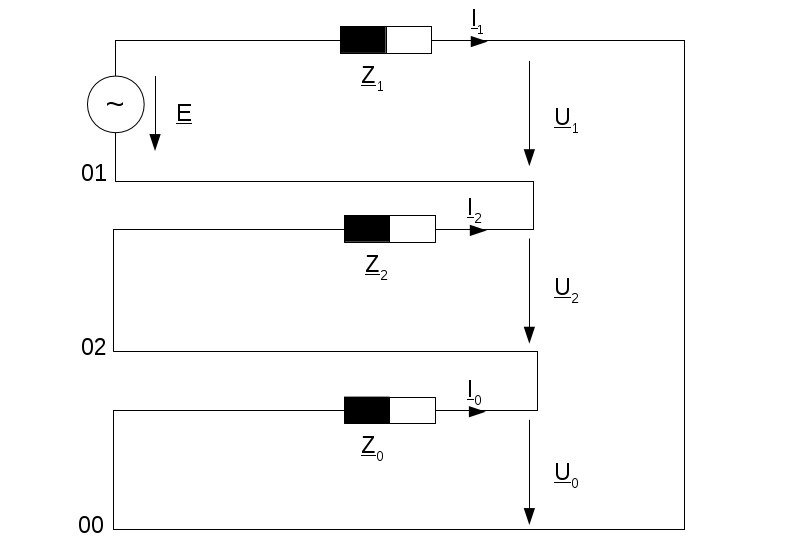
\includegraphics[scale=0.6]{img/einpol-fehler.png}
	\caption{Einpoliger Fehler in symmetrischen Komponenten}
	\label{einpol-fehler}
	\end{figure}
	
\subsubsection{Spannungserhöhung und Erdfehlerfaktor}
Zur Charakterisierung der Sternpunktbehandlung von elektrischen Netzen wird der Erdfehlerfaktor verwendet. Der Erdfehlerfaktor $\delta$ gibt dabei an, wie wirksam die Erdung der Sternpunkte ist. Eine Folge von einpoligen Fehlern ist die Erhöhung der Leiter-Erdspannung in den nicht fehlerbehafteten Leitern. Der Erdfehlerfaktor beschreibt dabei das Verhältnis zwischen der maximal auftretenden Leiter-Erdspannung $U_{LEmax}$ und der vor Fehlereintritt vorherrschenden Betriebsfrequenten Spannung $U^b$ geteilt durch $\sqrt{3}$. Ein Netz gilt dann als \glqq starr geerdet\grqq, wenn der Erdfehlerfaktor unter 1,4 bleibt. Gleichzeitig muss das Verhältnis von $X_0$ zu $X_1$ zwischen zwei und vier liegen \cite[S. 39]{Schlabbach2002}. Bei der strombegrenzenden Sternpunkterdung ist die Nullimpedanz wesentlich größer, der Erdfehlerfaktor liegt zwischen 1,4 und $\sqrt{3}$ \cite[S. 33 ff]{Schlabbach2002}.
% Das heißt, dass die Spannungsanhebung der fehlerfreien Leiter auf maximal das 1,4fache der vor Fehlereintritt auftretenden Spannung ansteigen darf. Dies wird vor allem bei Höchstspannungsnetzen angestrebt. Daraus lässt sich folgern, dass der Fehlerstrom umso höher ist, desto kleiner der Erdungswiderstand ist. Erhöht sich nun der Widerstand des Nullsystems, so lässt sich der Fehlerstrom verkleinern.

\subsection{Weitere Fehlerarten}
Neben dem dreipoligen und einpoligen Kurzschluss gibt es, wie bereits erwähnt, weitere Kurzschlussarten. Diese Fehler sind sogenannte \glqq Querfehler\grqq{}. Analog dazu werden Fehler, die durch Unterbrechung eines oder mehrerer Leiter entstehen, als \glqq Längsfehler\grqq{} bezeichnet.

\subsection{Übergangswiderstand und Störlichtbogen}
Die wenigsten Fehler in elektrischen Netzen sind sogenannte \glqq metallische Fehler\grqq, also Fehler ohne Übergangswiderstand. In Freileitungsnetzen entstehen die meisten Fehler durch Überschläge an Isolatoren, die beispielsweise durch Vogelnester oder Blitzeinschläge verursacht werden. Dadurch entsteht an der Fehlerstelle ein Störlichtbogen, dessen Impedanz nichtlinear ist. Diese ist stromabhängig und kann durch die Warrington-Formel beschrieben werden \cite[S. 143]{Ziegler2008}: \\

\begin{equation}
R_{LB} = \frac{28700 \cdot l_{LB}}{I_{LB}^{1,4}}
\end{equation}

\subsection{Automatische Wiedereinschaltung}
Da der Großteil der Fehler in Freileitungsnetzen auf Störlichtbögen zurückzuführen sind, hat sich dort das Konzept der automatischen Wiedereinschaltung, auch Kurzunterbrechung genannt, durchgesetzt. Dabei wird nach Erkennung eines Fehlers die Leitung abgeschaltet und nach einigen hundert Millisekunden bis Sekunden diese wieder eingeschaltet. Im Großteil der Fehlerfälle erlöscht dadurch der Lichtbogen und der Fehler wird dadurch beseitigt. Die Leitung kann wieder normal betrieben werden und man spricht von einer \glqq AWE mit Erfolg\grqq. Tritt nach dem Wiedereinschalten erneut ein Kurzschluss auf, wird die Leitung endgültig abgeschaltet. Man spricht dann von einer \glqq AWE ohne Erfolg\grqq. \\
Grundsätzlich wird zwischen einer dreipoligen und einpoligen Kurzunterbrechung unterschieden, wobei diese sich durch ihre Unterbrechungsdauer deutlich unterscheiden. Vor allem in den USA wird die AWE bei allen Fehlerarten dreipolig durchgeführt, in Europa dagegen, außer bei selten auftretenden dreipoligen Fehlern, überwiegend einpolig. Da bei einer einpoligen Kurzunterbrechung des fehlerbehafteten Leiters die fehlerfreien Leiter weiter Ströme und somit Energie in den benachbarten Leiter induzieren, muss diese länger sein als eine dreipolige Kurzunterbrechung. In der Regel beträgt die Unterbrechungsdauer einer dreipoligen AWE im Bereich von 0,3 bis 0,5 Sekunden. Bei der einpoligen AWE beträgt diese dagegen ca. eine Sekunde\cite[S. 66]{Ziegler2008}. Bei Kabelfehlern wird grundsätzlich keine AWE durchgeführt, da Kabelfehler in der Regel nicht von selbst wieder verschwinden. Bei hybriden Leitungen, also Leitungen mit Freileitungs- und Kabelabschnitten, wie z.B. die sich im Bau befindliche 380kV-Leitung Wesel-Meppen, kann durch die Analyse der Störschriebe beurteilt werden, ob sich der Fehler auf einem Freileitungs- oder Kabelabschnitt befindet. Befindet sich der Fehler auf einem Kabelabschnitt, so wird die AWE blockiert, da diese keinen Erfolg haben würde \cite{hybrid-ltg}.

\subsection{Größen der Synchronmaschine}
Wie bereits dargestellt, ist die Kurzschlussimpedanz nicht konstant. Die Ursache dafür ist vor allem das Verhalten der Synchronmaschine. Da in konventionellen Kraftwerken ausschließlich Synchrongeneratoren zum Einsatz kommen, bestimmen diese maßgeblich den Verlauf des Kurzschlussstromes. Daher wird im folgenden Abschnitt näher auf die Synchronmaschine und ihre Größen eingegangen.

\subsubsection{Aufbau der Synchronmaschine}
Eine Synchronmaschine besteht, wie eine Asynchronmaschine, aus einem Ständer und einem Läufer. Der Aufbau des Ständers ist analog zur Asynchronmaschine. Bei einer Polpaarzahl von Eins sind in einem räumlichen Abstand von 120\degree{} um den Läufer drei Wicklungen angeordnet. Bei höheren Polpaarzahlen entsprechend sechs, neun, usw. Beim Aufbau des Läufers wird zwischen Schenkelpol- und Vollpolläufern unterschieden. Kleine und langsam laufende Generatoren (Laufwasserkraftwerke) besitzen meist einen Schenkelpolläufer. In großen schnell drehenden Kraftwerksgeneratoren sind Vollpolläufer verbaut, da Schenkelpolläufer nicht die enormen Fliehkräfte aushalten können \cite[S. 508 ff]{Binder2012}
%\\ (el. netze u. kraftwerke: S. 126 ff)

\subsubsection{d-q-Achse}
Die Reaktanz einer Synchronmaschine setzt sich aus einem Anteil der Längsachse (d-Achse) und einem Anteil der Querachse (q-Achse) zusammen. Bei der Schenkelpolmaschine ist die magnetische Leitfähigkeit der d-Achse größer als die der q-Achse, was zur Folge hat, dass $X_d$ größer ist als $X_q$. Die ideale Vollpolmaschine ist mathematisch gesehen ein Sonderfall der Schenkelpolmaschine, bei der $X_d = X_q$ ist. Für eine einfache Kurzschlussstromberechnung sind die Reaktanzen der d-Achse ausreichend. Will man jedoch dynamische Vorgänge simulieren, so werden die Reaktanzen der q-Achse ebenfalls benötigt \cite[S. 184]{Heuck2007}. \\

	\begin{figure}[H]
	\centering
	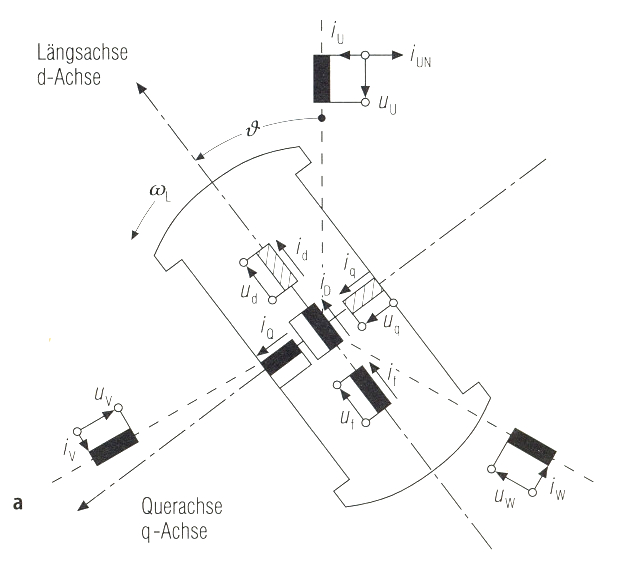
\includegraphics[scale=0.85]{img/schenkelpol.jpg}
	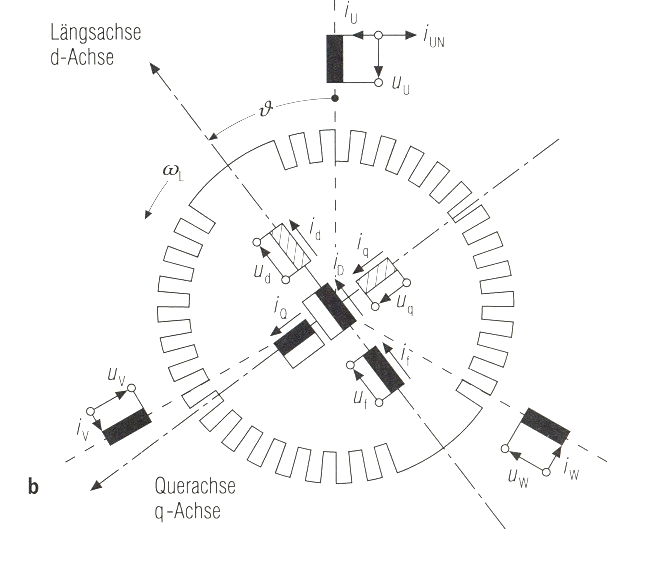
\includegraphics[scale=0.85]{img/vollpol.jpg}
	\caption{Querschnitt Schenkelpol- und Vollpolläufer \cite[S. 125]{Oeding2011} }
	\end{figure}

%	\begin{figure}[H]
%	\centering

%	\caption{test}
%	\end{figure}
%Ersetzt man nach der Zweiachsentheorie die drei Ständerwicklungen der Synchronmaschine durch zwei Ersatzwicklungen, so sind diese 90\degree elektrisch zueinander verschoben. Diese Komponenten auch als d-Achse (Längsachse) und q-Achse (Querachse) bezeichnet. Betrachtet man unsymmetrische Vorgänge, kommt noch eine 0-Komponente hinzu. Die Umrechnung der Drehstromkomponenten in dq0-Komponenten geschieht mit der Park-Transformation. Warum nur xd und kein xq bei KS-Berechnung?


\subsubsection{Subtransiente Reaktanz}
Um ersten Moment eines Kurzschlusses ist die subtransiente Reaktanz $X_d''$ wirksam. Mit ihr wird der Anfangskurzschlusswechselstrom berechnet. Ihr zugeordnet ist die subtransiente Zeitkonstante $T_d''$, welche das abklingen des Anfangskurzschlusswechselstromes beschreibt. Der Abklingvorgang wird mit einer e-Funktion beschrieben. Der gesamte subtransiente Vorgang dauert nur einige Halbwellen, danach geht der Kurzschluss in den transienten Vorgang über. Die Subtransientzeitkonstante $T_d''$ lässt sich wie folgt ermitteln: \\

$T_d'' = \frac{X_d'' + X_V}{X_d' + X_V} \cdot T_{d0}''$ \\

Dabei ist $T_{d0}''$ die Subtransient-Leerlaufzeitkonstante und liegt bei etwa 50ms. $X_V$ steht für die Netzimpedanz. Je höher die Netzimpedanz, desto größer ist auch die subtransiente Zeitkonstante \cite[S. 41]{Roeper1964}.



\subsubsection{Synchrone Reaktanz}
Die synchronen Reaktanz $X_d$ gibt die wirksame Reaktanz während des stationären Betriebs wieder. Sie ist auch nach dem Abschluss aller Ausgleichvorgänge wirksam, daher kann mit ihr der Dauerkurzschlussstrom ermittelt werden. Die Reaktanz der q-Achse wird entsprechend mit $X_q$ bezeichnet.

\subsubsection{Transiente Reaktanz}
Während des transienten Vorgangs, der wesentlich langsamer Abklingt als der subtransiente Vorgang, ist die transiente Reaktanz $X_d'$ wirksam.

\subsubsection{Gegensystem}
Die Gegenreaktanz der Synchronmaschine kann ungefähr aus dem Mittelwert von $x_d''$ und $x_q''$ bestimmt werden \cite[S. 165]{Funk1962} \\ \\
$x_i = \frac{x_d'' + x_q''}{2}$

\subsubsection{Nullsystem}
Da Synchronmaschinen symmetrisch aufgebaut sind, ist das Nullsystem theoretisch nicht wirksam. In der Praxis tritt die Nullreaktanz allerdings mit einer Größe von \\
$x_0 = \frac{1}{3} … \frac{1}{6} \cdot x_d'$ auf. Diese ist nur wirksam, wenn der Sternpunkt des Generators geerdet ist \cite[S. 166]{Funk1962}.

\subsubsection{Polradwinkel und Stabilität}
Der Polradwinkel, auch Lastwinkel genannt, gibt die Phasenverschiebung zwischen Polradspannung $U_p$ und Netzspannung an. Mechanisch gesehen ist er die mechanische Verschiebung des Polrads zwischen Leerlauf und Last. Jeder Leistung ist dabei ein Lastwinkel zugeordnet. Befindet sich die Maschine im Generatorbetrieb, eilt das Polrad vor und \glqq zieht\grqq{} das Netz mit. Arbeit die Maschine als Motor, eilt das Polrad nach und wird vom Netz \glqq mitgezogen\grqq \cite[S. 187]{Heuck2007}.

Das Kriterium der Stabilität eines elektrischen Netzes unterscheidet zwischen der statischen Stabilität und der transienten Stabilität. Die statische Stabilität beschreibt.

Der Polradwinkel eines Generators hat einen entscheidenden Einfluss auf die Stabilität.

Die transiente Stabilität beschreibt das Verhalten des Netzes im Moment eines Fehlereintritts und danach.

Treten in einem Netz Fehler auf, so ändern sich die Lastflussverhältnisse und somit auch die abgegebene Leistung der Generatoren. Ein Spannungseinbruch, beispielsweise als Folge eines Kurzschlusses, führt zu einem schlagartigen Abfall der Last an einem Generator. Da die elektrische Energie nun nicht mehr ins Netz abgeführt werden kann, an der Welle aber immer noch mechanische Energie zugeführt wird, wird diese mechanische Energie in Form von Rotationsenergie gespeichert, der Generator beschleunigt. Durch die Beschleunigung des Generators vergrößert sich der Polradwinkel. Wird dieser zu groß und überschreitet die Stabilitätsgrenze, gerät der Generator \glqq außer Tritt\grqq, wodurch es zu Schäden kommen kann. Diese liegt bei einem Polradwinkel von $\upsilon = 90\degree$ und markiert das Kippmoment $M_k$ der Maschine \cite[S.187]{Heuck2007}. Umso länger der Fehler andauert und umso näher der Fehler in der Nähe eines Genertors liegt, desto weniger Energie können die Generatoren ins Netz abführen. Die Wahrscheinlichkeit, dass ein Generator \glqq durchtritt\grqq, steigt also mit der Kurzschlussdauer an \cite[S. 56]{Nelles2009}. Generatornahe Fehler müssen daher besonders schnell abgeschaltet werden. Durch ein schnelles erhöhen der Generatorspannung kann erreicht werden, dass im Fehlerfall mehr Wirkleistung abgeführt werden kann. Kleinere Spannungsänderungen im Netz führen, wie bereits beschrieben, zu Leistungsänderungen an den Generatoren. Diese führen in der Regel nicht zu Instabilitäten, allerdings pendelt nun das Polrad mit einer niedrigen Frequenz von bis zu 2 Hz. Diese Leistungspendelungen sind auch im Netz beobachtbar, vor allem zwischen schwach gekoppelten Netzen. Sichtbar gemacht werden diese mit Wide Area Monitoring Systems \cite{wams-swissgrid}.

Die Stabilität eines Drehstromnetzes ist ein wesentliches Kriterium zur Versorgungssicherheit.

%- S. 902 \\
%- niederfrequente netzpendelungen \\
%- statisch \\
%- transient \\
%- Zeit zum durchgehen \\


\section{Simulation mit PSS Sincal}


\subsection{Lizenzen}
Die Fachhochschule Bielefeld besitzt unterschiedliche Lizenzen für die PSS Sincal Plattform. Mit allen Lizenzen können Kurzschlüsse, Lastflüsse und die Stabilität untersucht werden. Die EduTrans-Lizenz ist hier auf maximal 25 gleichzeitige Nutzer begrenzt. Mit dieser Lizenz können ferner Schutzfunktionalitäten und Oberschwingungen untersucht werden. Elektromagnetische Transienten und zeitliche Verläufe von Momentanwerten können allerdings nicht dargestellt werden. Die Lizenz EleStd ermöglicht dagegen auch die Untersuchung von elektromagnetischen Transienten und Eigenwerten. Hier fehlt allerdings Funktion der Schutzkoordination. EleStd ist auf sechs gleichzeitige Nutzer begrenzt. \\
Des weiteren verfügt die Fachhochschule über zwei EleKey2-Lizenzen, welche im Gegensatz zu den Netzwerklizenzen auf einen USB-Dongle setzt. Diese Lizenzen enthalten die selben Funktionen wie die EleStd-Lizenz. \\
Die lokale Auswahl der Lizenz erfolgt über das Programm \glqq PSS Tool\grqq.

\subsection{Versuchsnetz}
Das Netz, welches im Praktikum verwendet wird, ist im Anhang in Abbildung \ref{praktikum-netz} abgebildet. Es ist ein vermaschtes starr geerdetes 110kV-Freileitungsnetz. Als Einspeisequellen dienen zwei räumlich unterschiedlich angeordnete Synchrongeneratoren mit Leistungen von 100MVA und 80MVA, sowie das überlagerte 380kV-Netz. Die Netzdaten wurden von den Praktikumsunterlagen \glqq ENE 3 Kurzschlussstromberechnung in elektrischen Netzen\grqq{} übernommen. Die Dynamikdaten der Generatoren wurden aus den Praktikumsunterlagen der Otto-von-Guericke-Universität Magdeburg übernommen.

\subsection{Berechnungsmethoden}
PSS Sincal bietet unterschiedliche Berechnungsverfahren für unterschiedliche Zwecke an. Neben den drei geläufigsten Verfahren, Lastflussberechnungen, Kurzschlussberechnungen und Dynamikberechnungen, können auch Oberschwingungen und die Koordination von Schutzgeräten untersucht werden. Die Unterschiedlichen Lizenzen schalten unter anderem unterschiedliche Berechnungsmethoden frei, wobei Lastfluss- und Kurzschlussberechnungen in allen Lizenzen vorhanden sind.

\subsubsection{Lastfluss}
Mit Lastflussberechnungen lässt sich im Netz überprüfen, ob im fehlerfreien Betrieb Leitungen überlastet und Spannungsgrenzen eingehalten werden. Mit in die Berechnungen fließen auch modellierte Regler, wie beispielsweise Stufenschalter von Transformatoren oder Kompensationsanlagen, ein.

\subsubsection{Kurzschluss}
Kurzschlüsse können in Sincal wahlweise nach ANSI oder IEC 60909 bzw. VDE 0102 berechnet werden. Die Ergebnisse der Kurzschlussberechnung können zur Auslegung und Planung von Anlagen verwendet werden. Ergebnisswerte sind beispielsweise der Anfangskurzschlusswechselstrom oder der Stoßkurzschlussstrom. \\
Das Verfahren zur Berechnung von Kurzschlussströmen nach IEC 60909 bzw. VDE 0102 ist laut Norm für Netze bis 550 kV und 50 oder 60 Hz geeignet. Es ist besonders einfach gehalten und liefert doch ausreichend genaue Ergebnisse.


\subsubsection{Dynamik}
PSS Sincal benutzt für die Dynamikfunktionen im Hintergrund PSS NETOMAC. Dazu werden die Netztopologie, Fehleruntersuchungen und Plottdefinitionen automatisch beim Starten der Berechnungen exportiert. Diese befinden sich anschließend im Projektordner in einem separaten Ordner namens \glqq NETO\grqq.

Die Dynamikberechnungen bilden die mit Abstand größte Funktionsvielfalt in NETOMAC. Mit ihr lassen sich zum einen die Stabilität eines Netzes und zum anderen elektromagnetische Transienten berechnen und grafisch darstellen. Vor der eigentlichen Dynamikberechnung führt Sincal eine Lastflussberechnung durch, um Spannungen und Ströme im ungestörten Betrieb an den Knoten und Zweigen zu ermitteln. \\
Stabilitätsberechnungen und EMT-Berechnungen unterscheiden sich in ihrer Art der Berechnung. Während für Stabilitätsberechnungen das Netz mit komplexen Impedanzen und Regler und Maschinen mit Differentialgleichungen dargestellt werden, werden bei der Berechnung von elektromagnetischen Transienten alle Komponenten durch Differentialgleichungen dargestellt. Dies erlaubt die Lösung aller elektromechanischen und elektromagnetischen Phänomene \cite[Verfahrensbeschreibung $\rightarrow$ Dynamik]{netomac-hilfe}.

Ein weiterer Punkt, der auch zum Bereich der Dynamik eingeordnet werden kann, ist die Berechnung von Eigenwerten des Netzes \cite[S. 389]{Heuck2007}.

\subsection{Berechnungsparameter}
In dem Menü \glqq Berechnungsparameter\grqq{} lassen sich unter dem Reiter \glqq Dynamik\grqq{} verschiedene globale Parameter einstellen. So wird dort die Anfangs- und Endzeitpunkt der Berechnungen festgelegt, sowie die Größe des Zeitschritts. Bei kleineren Zeitschritten ist das Ergebnis zwar genauer, die Berechnungen dauern aber entsprechend länger. Außerdem kann angegeben werden, ob eine COMTRADE-Datei erzeugt werden soll, worauf später noch mehr eingegangen wird.

\subsection{Arbeitsbereich}
Änderungen in Berechnungsparametern oder in Beschriftungsfiltern werden für jedes Projekt separat als \glqq Arbeitsbereich\grqq{} gespeichert. Dieser kann exportiert und in anderen Projekten wiederverwendet werden. Das hat den Vorteil, dass in allen Projekten die gewünschte Ansicht sofort zur Verfügung steht. Als Beispiel sei hier die Anzeige von Berechnungsergebnissen von Kurzschlussberechnungen genannt. Es kann für jeden Netzelementtyp individuell festgelegt werden, welche Ergebnisse im Netzplan angezeigt werden sollen.

\subsection{Vierpoldarstellung von Leitungen}
Bei einfachen Kurzschlussstromberechnungen wird bei elektrischen Leitungen der Querzweig vernachlässigt und nur der Längszweig mit Induktivitäten und Resistanzen betrachtet. Dies führt bei der Auslegung von Betriebsmitteln zu hinreichend genauen Ergebnissen. Werden nun aber dynamische Vorgänge betrachtet, lassen sich die Querzweige nicht mehr vernachlässigen und müssen in die Betrachtungen mit einfließen.

%\subsubsection{Vollständiges Ersatzschaltbild}
%Das vollständige Ersatzschaltbild einer Leitung besteht aus v

\subsubsection{$\pi$-Ersatzschaltbild}
Bis zu einer Leitungslänge von ca. 150km liefert das $\pi$-Ersatzschaltbild ein realistisches Übertragungsverhalten. Bei längeren Leitungen müssen mehrere Pi-Glieder hintereinander geschaltet werden \cite[S. 216]{Heuck2007}. Der Vorteil am $\pi$-Ersatzschaltbild ist, dass es keine inneren Knoten besitzt und dadurch Rechnungen stark vereinfacht.

	\begin{figure}[H]
	\centering
	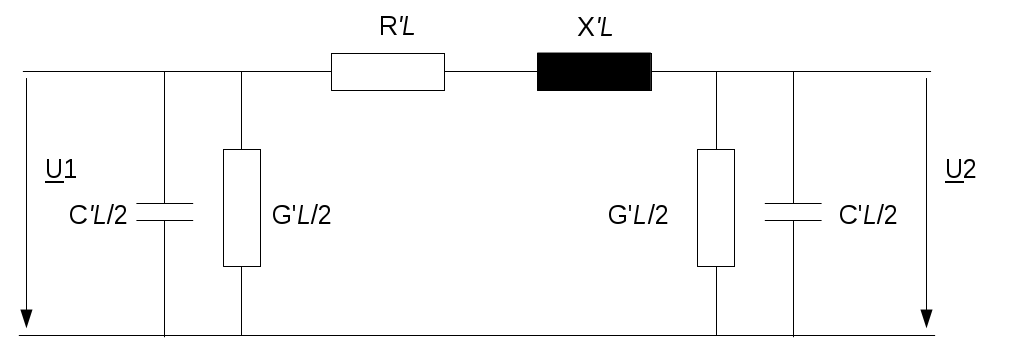
\includegraphics[scale=0.5]{img/pi-esb.png}
	\caption{$\pi$-Ersatzschaltbild Leitung}
	\label{pi-esb}
	\end{figure}

\subsubsection{T-Ersatzschaltbild}
Das $\pi$-Ersatzschaltbild hat bei dynamischen Betrachtungen den Nachteil, dass sich an seinen Enden Kapazitäten befinden, die im Kurzschlussfall zusammen mit der Induktivität einen nur schwach gedämpften Schwingkreis bilden. Dies führt bei der grafischen Darstellung zu \glqq Spikes\grqq{}, die in der Realität nicht vorkommen. Tritt dieser Fall auf, so liefert das T-Ersatzschaltbild realistischere Ergebnisse \cite[Verfahrensbeschreibung $\rightarrow$ Netzelemente]{netomac-hilfe}. Sichtbar wird dies bei einem Vergleich der Abbildungen \ref{u-pi} und \ref{u-t}. Diese zeigen den Spannungsverlauf bei einem dreipoligen Kurzschluss auf der Leitung L67 an der Sammelschiene SS6 des Praktikumnetzes. Wie zu erkennen, sind die \glqq Spikes\grqq{} beim T-Ersatzschaltbild wesentlich kleiner.

	\begin{figure}[H]
	\centering
	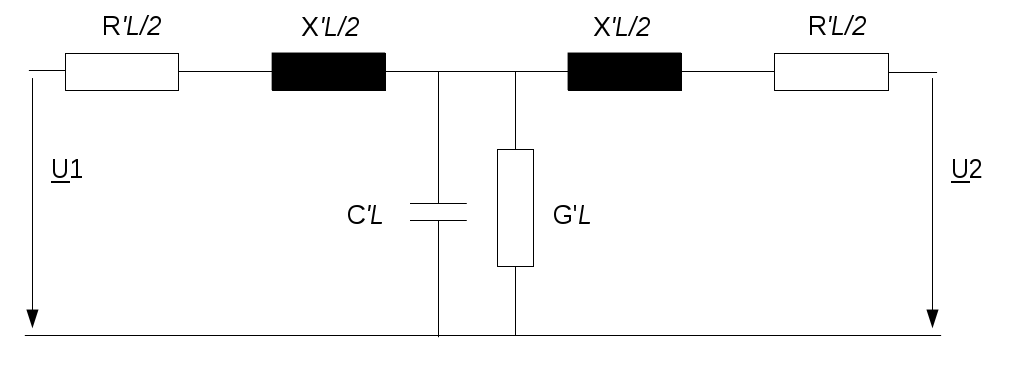
\includegraphics[scale=0.5]{img/t-esb.png}
	\caption{T-Ersatzschaltbild Leitung}
	\label{t-esb}
	\end{figure}
	
	\begin{figure}[H]
	\centering
	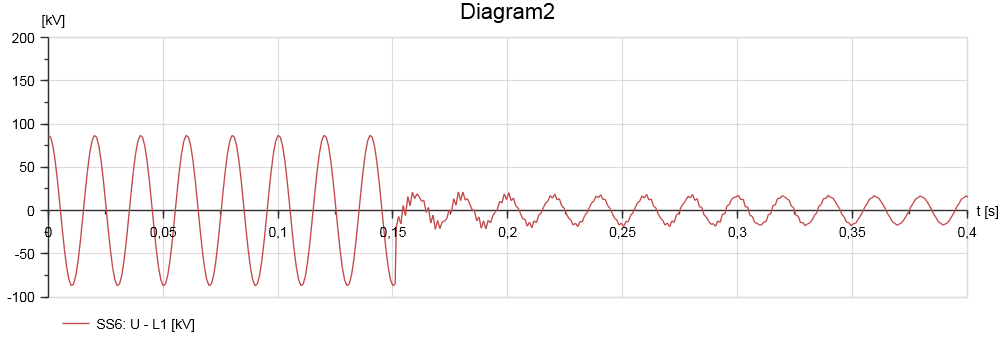
\includegraphics[scale=0.45]{img/u-pi.png}
	\caption{Spannung an SS6 mit PI-ESB}
	\label{u-pi}
	\end{figure}
	
	\begin{figure}[H]
	\centering
	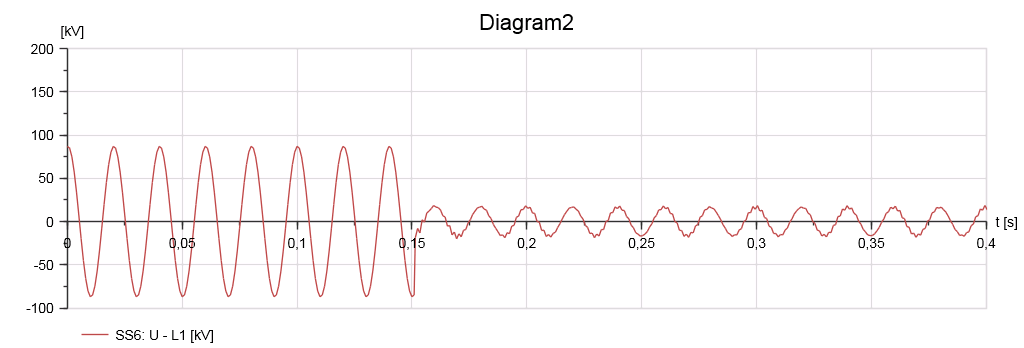
\includegraphics[scale=0.45]{img/u-t.png}
	\caption{Spannung an SS6 mit T-ESB}
	\label{u-t}
	\end{figure}

\subsection{Fehleruntersuchungen}
Soll an einer Leitung eine Fehleruntersuchung durchgeführt werden, so kann mit einem Rechtsklick unter dem Punkt Einfügen eine solche eingefügt werden. Es stehen sämtliche Fehlerszenarien zur Verfügung. Unter dem Punkt Dynamik können Fehlerbedingungen festgelegt werden, bei denen der Fehler ein- und ausgeschaltet werden soll. Diese können Zeit-, Strom oder Spannungsabhängig sein.

	\begin{figure}[H]
	\centering
	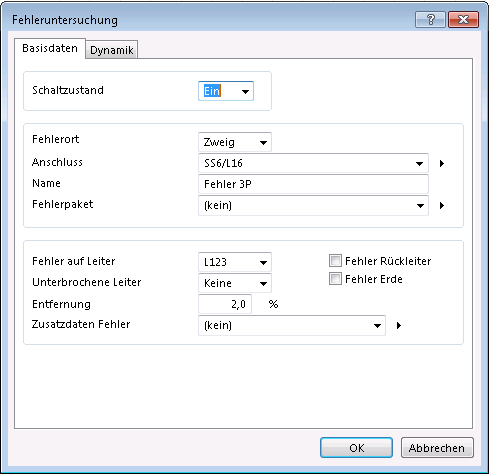
\includegraphics[scale=0.4]{img/fehleruntersuchung-basis.png}
	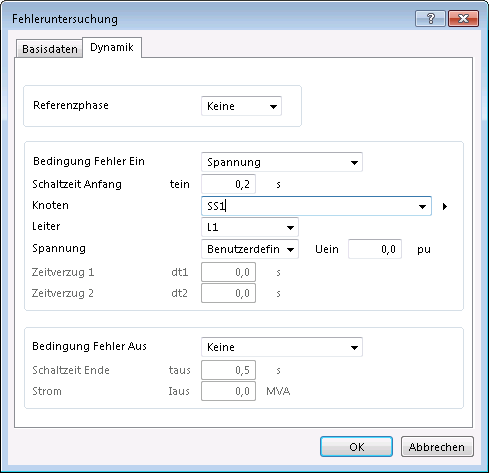
\includegraphics[scale=0.4]{img/fehleruntersuchung-dyn.png}
	\caption{Eingabedaten Fehleruntersuchung}
	\end{figure}

Um einen Fehler realistisch darzustellen, muss anschließend die vom Fehler betroffene Leitung vom Netz getrennt werden. Dies geschieht über die Funktion \glqq Elementschaltzeiten\grqq. Dort können, ähnlich wie beim Punkt Fehleruntersuchung, Bedingungen vorgegeben werden, wann eine Leitungsverbindungen aufgetrennt werden soll. Da auch ein Zuschalten möglich ist, lässt sich dadurch auch eine AWE simulieren. Unterschieden werden muss beim Punkt Schaltbedingung zwischen \glqq Standard\grqq{} und \glqq Zeitpunkt\grqq. Bei beiden Auswahlmöglichkeiten werden Schaltzeiten angegeben, bei \glqq Standard\grqq{} wird allerdings jede Phase erst individuell beim nächsten Spannungsnulldurchgang geschaltet. Nur wenn \glqq Zeitpunkt\grqq{} ausgewählt wird, werden alle Phasen zum selben Zeitpunkt geschaltet.

	\begin{figure}[H]
	\centering
	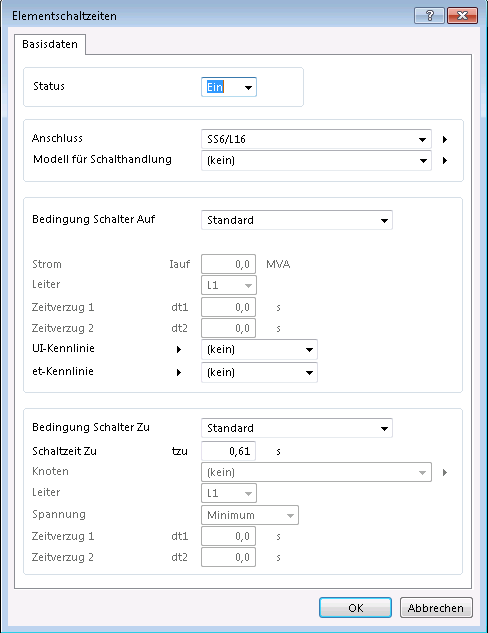
\includegraphics[scale=0.4]{img/elementschaltzeiten.png}
	\caption{Eingabedaten Elementschaltzeiten}
	\end{figure}
	
\subsection{Grafische Auswertung}
Zur grafischen Auswertung der Dynamikberechnungen müssen in Sincal unter dem Punkt $Daten \rightarrow Dynamik \rightarrow Plottdefinition$ entsprechende Signale definiert werden. Signale können Spannungen, Ströme, Leistungen aber auch Polradwinkel der Generatoren sein. Der Verlauf von Strömen an der Kurzschlussstelle kann nicht direkt dargestellt werden. Ähnlich wie in realen Umspannanlagen werden den Stromsignalen ein Knoten und ein Leitungsabgang zugeordnet. Es lassen sich also nur Teilkurzschlussströme darstellen. \\
Sind alle Signale generiert, werden diese nach einer Simulation in der Tabellenansicht auf Diagrammen zugeordnet. Dabei können in einem Diagramm auch mehrere Signale dargestellt werden.

	\begin{figure}[H]
	\centering
	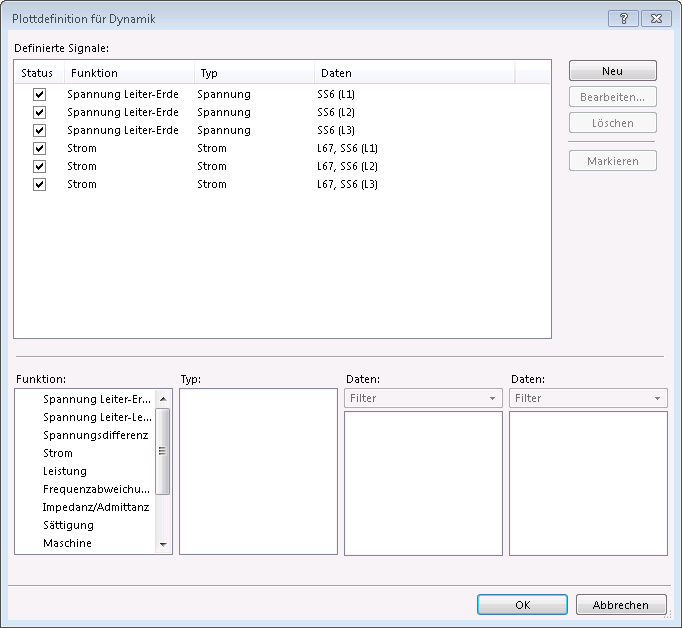
\includegraphics[scale=0.5]{img/plottdefinition.png}
	\caption{Plottdefinition}
	%\label{leitung-netomac}
	\end{figure}

\section{Simulation mit PSS NETOMAC}
PSS NETOMAC ist eine leistungsfähige Software zur Untersuchung von dynamischen Vorgängen in elektrischen Netzen. Es wird von der Firma Siemens entwickelt und vertrieben. Der Name NETOMAC steht für \textbf{Net}work \textbf{To}rsion \textbf{Ma}chine \textbf{C}ontrol und weißt auf den ursprünglichen Einsatzzweck hin. Mit ihm können nicht nur elektromagnetische Vorgänge in Netzen analysiert werden, sondern auch der Einfluss auf dieser auf die mechanische Belastung von Generatoren. Als Praxisbeispiel sei hier der Betrieb des Generators von Block A des Kernkraftwerkes Biblis als Phasenschieber genannt. Dort wurde dieser vor dem Umbau mit NETOMAC die Synchronisation mit dem Netz und der Blockschutz simuliert \cite{phasenschieber-biblis}.

\subsection{Export aus PSS Sincal}
Über die Exportfunktion von PSS Sincal lässt sich aus einem Sincal-Projekt ein NETOMAC-Projekt erstellen. Sie findet sich unter $Datei \rightarrow Exportieren \rightarrow PSS$ $NETOMAC...$ .  Nach dem erfolgreichen Export erhält man unter anderem  Dateien mit folgenden Dateiendungen:

\begin{itemize}
\item .nprj: Projektdatei
\item .ctl: Steuerungsdatei
\item .net: Hauptdatei mit Netzaufbau
\item .nzd: Datei mit Namen und Aliasnamen
\item .dis: Störungsdatendatei
\item .plo: Plotterdatendatei
\item .res: Ergebnisdatei
\end{itemize}


\subsection{.ctl-Datei}
In der .ctl-Datei werden allgemeine Einstellungen festgelegt, wie z.B. der Simulationszeitraum und der Zeitschritt. Des weiteren werden dort die Suchpfade festgelegt, in denen NETOMAC benötigte Dateien suchen soll.

\subsection{.net-Datei}
In der .net-Datei sind alle Betriebsmittel, Knoten und Zweige und die Netztopologie definiert. Jedes Betriebsmittel und jeder Knoten hat eine eindeutige Bezeichnung, aus der nicht direkt ersichtlich ist, um welche Art von Betriebsmittel es sich handelt. In jeder Definition eines Betriebsmittels sind der Anfangsknoten und der Endknoten definiert. Nachfolgend ist in Tabelle \ref{leitung-netomac-tb} die Definition einer Leitung dargestellt, an der die Funktionsweise von NETOMAC demonstriert wird.

\begin{table}[H]
\begin{tabular}{|l|l|l|l|l|l|l|l|l|l|l|l|}
\hline 
\multicolumn{12}{|l|}{\$ Line: L12 (X00028) from SS1 (X00005) to SS2 (X00006)} \\ 
\hline 
LX00005 & X00006  & X00028 & 1 & 30 & 0.116 & 0.424 & 9.17 & 0 & 110 & 0 &0 \\ 
\hline 
M & & X00028 & & 9999 & 9999 & & & & & & \\ 
\hline 
\end{tabular} 
\caption{Definition einer Leitung in PSS NETOMAC}
\label{leitung-netomac-tb}
\end{table}

NETOMAC arbeitet mit einem tabellenartigen Textformat, Spalten sind dabei durch Tabulatoren getrennt. Die Kennzeichnung von Zeilen geschieht durch Buchstaben, wobei jeder Buchstabe eine andere Funktion hat. Die Eigenschaften der Zeile wird anschließend in den Spalten festgelegt.

Alle Zeilen, die mit einem \$ beginnen, sind Kommentare. Beim Export von PSS Sincal in PSS NETOMAC versieht Sincal automatisch alle Betriebsmittel mit Kommentaren. Knoten- und Betriebsmittelkennzeichnungen beginnen mit X und haben eine eindeutige alphanumerische Bezeichnung. In diesem Beispiel hat die Leitung L12 die Bezeichnung X00028 und verbindet die Knoten X00006 und X00028 miteinander. Die Zeile mit der Bezeichnung L kennzeichnet eine Leitung, anschließend folgt ohne Leerzeichen die Bezeichnung des Anfangsknotens (X00005). In der nächsten Spalte folgt nach einem Tabulator die Bezeichnung des Endknotens (X00006), anschließend die Bezeichnung der Leitung selbst. Ab hier beginnen die eigentlichen Parameter der Leitung. Zunächst wird die Anzahl der parallelen Leitungen festgelegt, in diesem Fall 1. Die Länge ist mit 30km definiert. Anschließend werden die Resistanz R' mit 0,116 $\Omega /km$, die Reaktanz mit 0,424 $\Omega /km$ und die Kapazität $C_b'$ mit 9,17nF/km festgelegt. Da in der Versuchsbeschreibung kein Wert für $C_0'$ gegeben war, ist dieser Null. Die Nennspannung auf der Leitung beträgt 110kV. Für die Ableitwiderstände gilt dasselbe wie für $C_0'$, daher wurden $G_1'$ und $G_0'$ auch zu Null.\\
In der Zeile mit der Bezeichnung M wird die Kopplung zwischen dem Mit- und Nullsystem definiert. Spalte zwei und drei sind leer, in der vierten Spalte wird die Bezeichnung der Leitung angegeben, für die die Kopplung definiert werden soll, in diesem Fall X00028. Da auch hier keine Werte gegeben sind, setzt Sincal die beiden folgenden Spalten, welche für das Verhältnis $R_0'/R_b'$ und $X_0'/X_b'$ stehen, auf 9999. Das bedeutet, dass die beiden Werte für $X_0'$ und $R_0'$ praktisch nicht vorhanden sind. Nachfolgend ist in Abbildung \ref{leitung-netomac} die Leitung L12, wie in Tabelle \ref{leitung-netomac-tb} beschrieben, noch einmal im Texteditor von NETOMAC dargestellt.

	\begin{figure}[H]
	\centering
	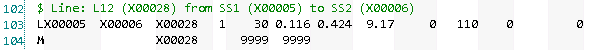
\includegraphics[scale=0.75]{img/netomac-l12.png}
	\caption{Definition der Leitung L12 in NETOMAC}
	\label{leitung-netomac}
	\end{figure}
	
Da in die Betriebsmittelbezeichnungen in der .net-Datei kryptisch und ohne Bezug sind, hat NETOMAC die Möglichkeit von Aliasnamen eingeführt. Diese sind in der Datei mit der Endung .nzd definiert. PSS Sincal legt automatisch Aliases mit den in Sincal angegebenen Namen an. \\
Generatoren werden nach dem selben Prinzip beschrieben. Zeile S kennzeichnet eine Synchronmaschine. Da dieses Betriebsmittel keinen Anfangs- und Endknoten hat, bleiben die nachfolgenden zwei Spalten leer. In der dritten Spalte folgt wie üblich die Bezeichnung des Betriebsmittels. Zeile T legt die Transformator-Parameter fest. Da der Generator und der Transformator separat betrachtet werden und nicht als Kraftwerksblock, ist das Übersetzungsverhältnis 1. Die Schaltgruppe des Synchrongenerators ist YY0, was bedeutes, dass die Ständerwicklungen im Stern verschaltet sind. Da das Übersetzungsverhältnis 1 ist, sind die nachfolgenden Angaben für $U_{r,UStrafo}$, $U_{nUStrafo}$ und $U_{nOSnetz}$ jeweils 10kV. Die Bemessungsspannung des Synchrongenerators beträgt allerdings 10,5kV. Die nachfolgende Zeile definiert die Nennwerte der Maschine. Auf die Scheinleistung in MVA folgt die Wirkleistung, die Nennspannung, der Leistungsfaktor, der Wirkungsgrad, die Nenndrehzahl und die Nennfrequenz. In Zeile zwei bis sechs sind die Parameter des Ersatzschaltbildes der Maschine definiert. Die Z-Zeile beinhaltet weitere Parameter, die zur Kurzschlussberechnung nach IEC und ANSI benötigt werden.

	\begin{figure}[H]
	\centering
	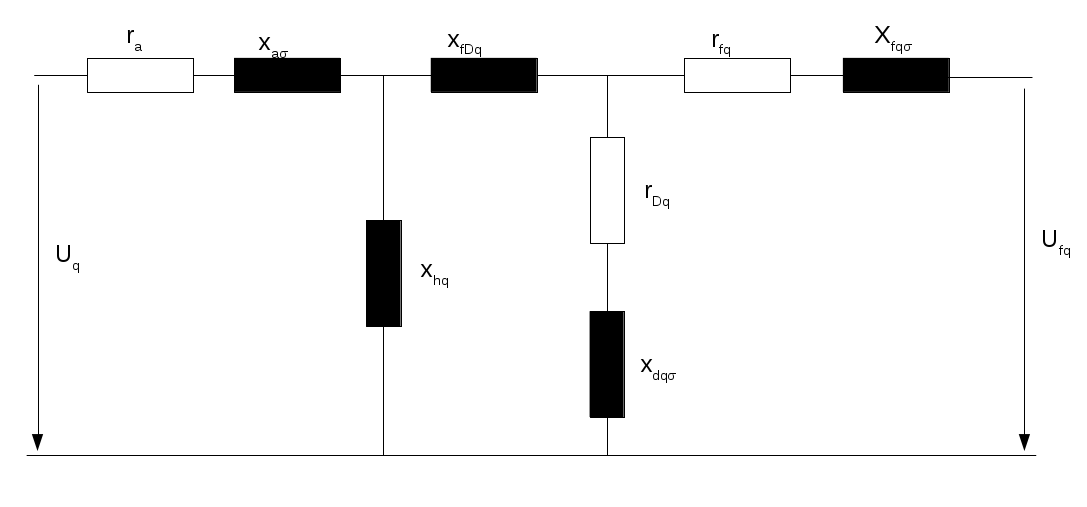
\includegraphics[scale=0.5, trim=0cm 1.5cm 0cm 1cm, clip]{img/esb-synchron.pdf}
	\caption{Ersatzschaltbild Synchrongenerator}
	\label{leitung-netomac}
	\end{figure}

	\begin{figure}[H]
	\centering
	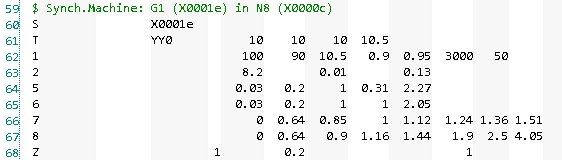
\includegraphics[scale=0.75]{img/netomac-g1.png}
	\caption{Definition des Synchrongenerator G1 in NETOMAC}
	\label{leitung-netomac}
	\end{figure}

\subsection{.dis-Datei}
In der .dis-Datei (\glqq disturbance\grqq) werden die Störkriterien und Netzänderungen festgelegt. Einzelne Ereignisse können dabei sequenziell oder parallel ablaufen. Jedes Ereignis kann aus mehreren Störkriterien bestehen und beginnt mit einer Einleitungszeile. Die Einleitungszeile dient dazu, NETOMAC kenntlich zu machen, das ein neues Ereignis stattfindet. In ihr wird die Zeit angegeben, nach der das nächste Ereignis ausgeführt werden soll. Nach der Einleitungszeile folgen Fehlerzeilen. Jede Fehlerzeile definiert dabei den Fehlerort, die Art des Fehlers, die Fehlerimpedanz und eventuell eine Fehlerimpedanz gegenüber Erde. Das Ereignisende erfolgt eine \glqq ENDE\grqq -Zeile. Nun kann das nächste Ereignis definiert werden. Soll das Netz in den Ausgangszustand zurückversetzt werden, geschieht dies mit einer \glqq OLD\grqq -Zeile, gefolgt von einer \glqq ENDE\grqq -Zeile. 

\subsection{.plo-Datei}
In der Plotterdatei wird definiert, welche Signale aufgenommen werden sollen. Dies kann auch komplett über ein grafisches Menü geschehen, was wesentlich komfortabler ist als die reine Texteingabe. Anschließend können, ähnlich wie in Sincal, über den \glqq Signalexplorer\grqq und die Diagrammansicht aufgenommene Signale grafisch dargestellt werden.

%\subsection{.res-Datei}

%\subsection{Dateistruktur}
%\subsection{Eingabedaten}


%\subsection{Festlegen der Störkriterien}
%\subsection{Grafische Auswertung}


\section{COMTRADE}
Das COMTRADE-Datenformat ist ein Standard zum Aufzeichnen von transienten Signalen, beispielsweise von Störungen in elektrischen Netzen. Diese können dann mit gängigen Programmen grafisch dargestellt und weiterverarbeitet werden. Eine Anwendungsmöglichkeit ist die Fehleranalyse von Störungen, die durch ein Versagen des Schutzgerätes verursacht werden. Dazu wird mit einem Prüfgerät, z.B. mit einem Kocos Artes oder einer Omicron CMC, die COMTRADE-Datei der Störung \glqq abgespielt\grqq{} und die Spannungen und Ströme auf das vermeintlich defekte Schutzgerät gegeben. So lassen sich die Auslösekennlinien im Labor mit echten Daten überprüfen. Die Analyse der Störung im Übertragungsnetz in der Region Trier im Jahr 2004 erfolgte mit digitalen Störschrieben der Schutzgeräte. Dort löste nach einem Fehler auf einer 220kV-Leitung ein elektromechanisches Schutzgerät einer anderen Leitung wahrscheinlich durch eine Schutzüberfunktion und Leistungspendelung aus, was zu einem Stromausfall in der Region Trier und Luxemburg führte \cite{abschlussbericht-trier}. \\ Da die Fachhochschule sowohl über ein solches Prüfgerät vom Typ Kocos Artes 460, als auch über verschiedene Schutzgeräte der aktuellen SIPROTEC-Reihe von Siemens verfügt, ist das Simulieren solcher Szenarien ohne weitere Hard- und Software möglich.

Ein COMTRADE-Datensatz kann aber auch durch Simulationen erzeugt werden. PSS Sincal und PSS NETOMAC bieten eine entsprechende Ausgabe an. Diese können anschließend zur Überprüfung von komplexen Schutzaufgaben im Labor verwendet werden.

Es existieren zwei Standards für das Format von COMTRADE-Dateien: C37.111-1991 und C37.111-1999, wobei C37.111-1999 der geläufigste ist. Die Standardbeschreibung kann über die Plattform IEEEXplore heruntergeladen werden \cite{ieee-comtrade}. \\
Im folgenden soll weiter auf den Aufbau von COMTRADE und dessen praktische Verwendung eingegangen werden.

%(Software zur Weiterverarbeitung)
\subsection{COMTRADE-Dateien}
Zu einem COMTRADE-Datensatz gehören folgende Dateien:

\begin{itemize}
\item .cfg
\item .dat
\item .hdr
\item .inf
\end{itemize}

Benötigt werden davon laut dem Standard von 1991 die Dateien mit den Endungen .cfg, .dat und .hdr. Im Standard von 1999 ist die .hdr-Datei optional, genauso wie die .inf-Datei, die erst mit diesem eingeführt wurde. Um die zusammengehörenden Dateien eines Datensatzes zu erkennen, muss der Dateiname gleich sein. Zur Datei NETWORK.CFG gehören also NETWORK.DAT, NETWORK.HDR und NETWORK.INF.

In .cfg-Datei befindet sich die Konfiguration im ASCII-Format. Dort werden die aufgezeichneten Signale, deren Bezeichnungen und Einheiten definiert. Ein Zeitstempel markiert den Beginn der Aufzeichnung. In der .dat-Datei befinden sich die eigentlichen Aufzeichnungsdaten. Diese können entweder im ASCII-Format oder im Binärformat vorliegen. In der .hdr-Datei können zusätzliche Informationen gespeichert werden. Sie ist im Standard von 1999 optional, im Standard von 1991 notwendig.

\subsubsection{.cfg-Datei}
Die Angaben in der .cfg-Datei sind aufgeteilt in \glqq kritisch\grqq{} und \glqq nicht kritisch\grqq. \glqq Kritisch\grqq{} bedeutet, dass eine Angabe vorhanden sein muss, \glqq nicht kritisch\grqq{} bedeutet, dass die Angabe optional ist. Sämtliche Parameter werden durch Kommata getrennt, ähnlich einer .csv-Datei. Die Parameter müssen in der richtigen Reihenfolge angegeben werden und es dürfen auch keine Zeilen vertauscht werden. \\
In der ersten Zeile befindet sich der Stationsname des Umspannwerks von dem die Aufzeichnung stammt. Der zweite Parameter, die \textit{rec\_dev\_id}, ist die Bezeichnung des aufzeichnenden Gerätes im Umspannwerk, damit identifiziert werden kann, um welchen Leitungsabgang es sich handelt. Der dritte Parameter ist Version des COMTRADE-Standards, der verwendet wird. Fehlt dieser Parameter, wird dies automatisch als Standard von 1991 interpretiert. In der zweiten Zeile gibt die erste Zahl die Gesamtanzahl der aufgezeichneten Kanäle an. Anschließend werden die Anzahl der analogen Signale und die Anzahl der binären Signale (Statussignale) angegeben. Im Beispiel in Abbildung \ref{bsp-cfg} sind dies zwei analoge Signale. Anschließend folgt für jedes Signal eine Zeile mit Parametern, in denen unter anderem der Signalname, Messeinheit und Messwandlerwerte angegeben sind. Nachdem alle analogen Kanäle definiert sind, folgen die Statuskanäle, die in dem Beispiel in Abbildung \ref{bsp-cfg} fehlen. In Statuskanälen können binäre Signale dargestellt werden, beispielsweise die Auslösung eines Schutzrelais. Als nächstes wird die Nominalfrequenz, in der Regel also 50 Hz, festgelegt. Die Definition der Samplingrate besteht aus mindestens zwei Zeilen. In der ersten Zeile wird die Anzahl der verschiedenen eingesetzten Samplingraten angegeben, anschließend folgen in den anderen Zeilen die Samplingrate in Hertz und als zweiter Parameter die Nummer des letzten Samples, die diese Samplerate benutzt. Die folgenden zwei Zeitstempel legen den Start- und Endpunkt der Aufzeichnung fest. Als letztes ist angegeben, in welchem Datenformat die Daten abgespeichert wurde. Die Angabe lautet entsprechend \glqq ASCII\grqq{} oder \glqq BINARY\grqq.

\begin{figure}[H]
\textit{COMTRADE file written by PSS®NETOMAC,1,1998 \\
002,002A,000D \\
1,SS6|U - L1|,,8,kV,0.0026687863,-87.4495010376,0.0000000000,0,065535,1.0,1.0,S \\
2,L67|I - SS6 - L1,,,kA,0.0000130651,-0.4281093180,0.0000000000,0,065535,1.0,1.0,S \\
50.0 \\
1 \\
10000.0000,10001 \\
29/07/2016,10:34:17.900000 \\
29/07/2016,10:34:17.900000 \\
ASCII \\
1.000000}
\caption{Beispiel einer .cfg-Datei}
\label{bsp-cfg}
\end{figure}

\subsubsection{.dat-Datei}
In der .dat-Datei befinden sich die eigentlichen Daten der Aufzeichnung. Diese können entweder im ASCII-Format oder im Binärformat vorliegen, je nachdem wie dies in der .cfg-Datei definiert ist. \\
Der Aufbau im ASCII-Format ist relativ simpel. Sofern die Samplerate aller Kanäle gleich ist, enthält jede Zeile Werte für jeden Kanal. Diese sind durch Kommata getrennt. Der erste Spalte bezeichnet die fortlaufende Samplenummer, die zweite Spalte bezeichnet den relativen Zeitpunkt. In den nachfolgenden Spalten stehen die Werte der analogen Kanäle. Wurden auch Statuskanäle aufgezeichnet, folgen diese nach den analogen Kanälen. \\
Liegen die Daten im ASCII-Format vor, können diese auch relativ einfach in Microsoft Excel kopiert und grafisch dargestellt werden.

\begin{figure}[H]
\textit{0000000001,0000000000,065433,065282 \\
0000000002,0000000100,065487,065387 \\
0000000003,0000000200,065502,065454}
\caption{Beispiel einer .dat-Datei mit zwei Signalen}
\end{figure}

\subsection{Erzeugen von COMTRADE-Dateien mit Sincal und NETOMAC}
Die Ergebnisse von mit NETOMAC durchgeführten Dynamiksimulationen lassen sich in das COMTRADE-Format exportieren. Dazu wird unter \textit{Berechnen $\rightarrow$ Parameter... $\rightarrow$ Ausgabe} die Einstellung \glqq COMTRADE Datei erzeugen\grqq{} aktiviert. Diese kann entweder Binär oder im ASCII-Format sein. In Sincal ist die entsprechende Funktion unter \textit{Berechnen $\rightarrow$ Parameter... $\rightarrow$ Dynamik} zu finden. Bei der nächsten Simulation finden sich die COMTRADE-Dateien nun in einem Unterordner namens COMTRADE.

Die von PSS Sincal erzeugten COMTRADE-Dateien haben leider das Problem, dass in diesen Angaben zur Einheit des Stroms fehlen und diese in der .cfg Datei manuell ergänzt werden müssen. Der Support teilte mit, dass der Grund dafür zu lange Signalbezeichnungen sind, die aus der kompletten Topologie von Sincal generiert werden. Daher müssen die .cfg-Dateien von Hand bearbeitet werden. Eine weitere Möglichkeit wäre, die Signalnamen in der von Sincal generierten .plo-Datei zu ändern und anschließend die Berechnung direkt in NETOMAC auszuführen, was aber deutlich aufwändiger ist. Durch ausprobieren in NETOMAC wurde eine Begrenzung der Signalnamen auf eine Länge von zwölf Zeichen festgestellt.

Ein weiteres Problem ist, dass NETOMAC ein falsches Zeitstempelformat in der .cfg-Datei verwendet. Im Standard C37.111-1999 ist \textit{dd/mm/yyyy,hh:mm:ss.ssssss} vorgesehen, NETOMAC verwendet jedoch \textit{mm/dd/yyyy,hh:mm:ss.ssssss} aus dem Standard C37.111-1991. Dies führt bei der Weiterverarbeitung zu Problemen. Während SIGRA und OMICRON die Datei akzeptieren und lediglich das Datum falsch angezeigt wird (07.12.2016 anstatt 26.07.2016), verweigert die Software Kocos Artes den Import der Datei und bricht mit einer nichtssagenden Fehlermeldung ab.
%Ein weiteres Problem ist, dass die Software von Kocos keine .cfg-Datei öffnen kann, in denen in der ersten Zeile der Parameter \glqq rec\_dev\_id\grqq{} verwendet wird. Dieser muss ebenfalls von Hand gelöscht werden. Die Software von Kocos hat auch Probleme, wenn die Daten im Binärformat vorliegen, daher sollten die COMTRADE-Daten im ASCII-Format erzeugt werden. Die Probleme zeigen sich in falsch dargestellten Signalen. woran dies liegt, konnte nicht geklärt werden.

\subsection{Anpassen der fehlerhaften COMTRADE-Datei}
PSS Sincal bietet die Möglichkeit, Scripte zum Automatisieren von Aufgaben einzubinden. Als Scriptsprachen stehen VBScript und Python zur Verfügung.

Da der Support von Sincal und NETOMAC keine Lösung für diese Probleme anbieten konnte und eine Behebung dieser wahrscheinlich erst in späteren Versionen erfolgt, wurde mit VBScript ein Script geschrieben, dass die Einheit für den Strom ergänzt und das Datum korrigiert. Der Quellcode befindet sich auf der DVD und im Internet unter \url{https://github.com/bodems/comtrade-adjust}. \\
Das Script initialisiert als erstes das aktuell geöffnete Sincalprojekt, liest daraus den absoluten Pfad der Datenbankdatei und speichert diesen in einer Variablen. Als nächstes muss dieser absolute Pfad angepasst werden damit er auf die .cfg-Datei von NETOMAC zeigt. Dazu wird der immer gleich bleibende Datenbankdateiname im Pfad abgeschnitten und an diesen \textit{\glqq NETO\textbackslash COMTRADE\textbackslash NETWORK.CFG \grqq{}} angehangen. Nun zeigt die Pfadvariable auf die von Sincal erzeugte .cfg-Datei. Diese wird nun eingelesen und anschließend gelöscht. Anschließend liest das Script aus der zweiten Zeile die Anzahl der Signale aus und überprüft in den nachfolgenden Signalzeilen, ob dort eine Einheit nach dem fünften Komma definiert ist. Ist das Zeichen nach dem fünften Komma ebenfalls ein Komma, so wird zwischen diesen die Einheit \glqq kA\grqq{} ergänzt. Sind alle Signalzeilen korrigiert, so sucht das Script nach einem \glqq /\grqq, welches als Formatierungszeichen für das Datum verwendet wird. Im Datum werden nun der Tag und der Monat vertauscht, dies geschieht in der nachfolgenden Zeile ein weiteres mal (Zeitstempel Anfang, Zeitstempel Ende). Als letztes wird nun der korrigierte Inhalt zurück in die NETWORK.CFG geschrieben. \\
Über den Menüpunkt \textit{Extras $\rightarrow$ Optionen $\rightarrow$ Makros} kann in Sincal das Verzeichnis konfiguriert werden, in dem sich die Scripte befinden. Anschließend kann dieses über \textit{Extras $\rightarrow$ Makro $\rightarrow$ Makros…} bequem nach jeder Dynamiksimulation ausgeführt werden. Da Windows generell keine Scripte ausführt, die sich auf Netzlaufwerken befinden, müssen Scripte auf der lokalen Festplatte gespeichert werden. Dazu bieten sich der Ordner \textit{C:\textbackslash Users\textbackslash Public\textbackslash Documents} an, da auf diesen Ordner alle Benutzer Leserechte haben. \\
Über Extras \textit{$\rightarrow$ Optionen $\rightarrow$ Benutzermenüs} kann das Makro auch direkt mit einem eigenen Menüpunkt dargestellt werden. Dieser neue Menüpunkt findet sich dann unter \glqq Extras\grqq.
\begin{figure}[H]
\textit{COMTRADE file written by PSS®NETOMAC,1,1998 \\
002,002A,000D \\
1,SS6|U - L1|,,8,kV,0.0027409648,-89.8145065308,0.0000000000,0,065535,1.0,1.0,S \\
2,L67|I - SS6 - L1,,\colorbox{yellow}{,,}0.0000508286,-1.6914786100,0.0000000000,0,065535,1.0,1.0,S \\
50.0 \\
3 \\
10000.0000,1002 \\
20000.0000,1003 \\
10000.0000,5001 \\
\colorbox{yellow}{08/30}/2016,12:14:14.450000 \\
\colorbox{yellow}{08/30}/2016,12:14:14.450000 \\
ASCII \\
1.000000}
\caption{Fehlerhafte .cfg-Datei}
\end{figure}

\subsection{Weiterverarbeitung}
Die korrigierten COMTRADE-Daten können anschließend mit Software verschiedener Hersteller weiterverarbeitet werden. Im Softwarepaket DIGSI der Firma Siemens, welches zur Konfiguration von Schutzgeräten dient, wird das Programm SIGRA mitgeliefert. Es enthält umfangreiche Analysefunktionen zur Auswertung von Störschrieben, z.B. die Darstellung der Daten als Zeigerdiagramm oder eine Fourieranalyse \cite{siemens-sigra}. \\
Die Firma Kocos liefert in ihrer Prüfsoftware das Modul TRANSIG mit. Mit ihr können COMTRADE-Dateien angezeigt, Signale bearbeitet und mit einem Prüfgerät der Serie Kocos Artes wiedergegeben werden \cite{kocos-transig}. Das entsprechende Pendant des Konkurrenten OMICRON heißt TransView \cite{omicron-transview}.

%\subsubsection{Abspielen von COMTRADE-Dateien mit Prüfgerät Kocos ARTES}
Nachdem die COMTRADE-Datei korrigiert wurde, kann diese nun in TRANSIG geöffnet werden. In TRANSIG werden den Signalen anschließend Spannungs- und Stromausgänge zugewiesen und der in Sincal simulierte und aufgezeichnete Kurzschluss kann auf ein Schutzrelais ausgegeben werden. Mit einem integrierten Signaleditor lässt sich die COMTRADE-Datei in TRANSIG auch noch nachträglich bearbeiten. \\
Es zeigte sich, dass TRANSIG Probleme mit COMTRADE-Daten im Binärformat hat. Signale werden verfälscht dargestellt, der Grund dafür ist nicht bekannt. SIGRA stellt dagegen Daten im Binärformat richtig dar. Liegen die Daten im ASCII-Format vor, werden die Signale auch in TRANSIG richtig dargestellt. \\
Nun kann jedem Signal ein Ausgang des Prüfgerätes zugeordnet werden. Da die aufgezeichneten Daten Primärwerte sind, das Prüfgerät aber mit Sekundärwerten arbeitet, müssen anschließend die Übersetzungsverhältnisse der Wandler konfiguriert werden.

Die Strom- und Spannungsausgänge des Prüfgerätes Kocos Artes 460 können transiente Signale bis zu einer Frequenz von 4 kHz bei einer Frequenzauflösung von 0,001 Hz erzeugen. Die Genauigkeit ist kleiner als 0,01\%. Die Auflösung der Spannungsausgänge liegt bei 13 mV bei einer Genauigkeit von unter 0,05\%. Die Stromausgänge weisen eine Auflösung von 1 mA und eine Genauigkeit von unter 0,05\% auf \cite[S. 35]{artes-brochuere}.


\subsection{Beispiel Fehlerortung mit Distanzschutz und COMTRADE}
Um den ganzen Vorgang auszuprobieren wurde mit Sincal ein 110 kV Netz modelliert, welches nur aus einer Einspeisung, einer 20 km langen Leitung und einer Last besteht. Die Parameter wurden aus dem Laborpraktikum übernommen. Auf der Leitung wurde anschließend ein dreipoliger Fehler eingefügt, mit unterschiedlichen Entfernungen Fehler simuliert und als COMTRADE exportiert. Mit der Software TRANSSIG wurden diese nun mit dem Kocos Artes 460 auf das digitale Distanzschutzgerät vom Typ 7SA87 der Firma Siemens gegeben. Die Parametrierung dieses mit der Software DIGSI übernahm zuvor Herr Michael Nollek. \\
Der Fehlerorter des Distanzschutzes berechnete die Entfernung allerdings nicht richtig. Bezogen auf die Länge bis zur Fehlerstelle wurde stets 7\% bis 9\% zu wenig angezeigt. Wurde mit Sincal ein Fehler bei 82\% (16,4 km) Entfernung simuliert, zeigte der Fehlerorter der Störaufzeichnungen eine Entfernung von 15,1 km an. Der Grund dafür konnte noch nicht ermittelt werden.

	\begin{figure}[H]
	\centering
	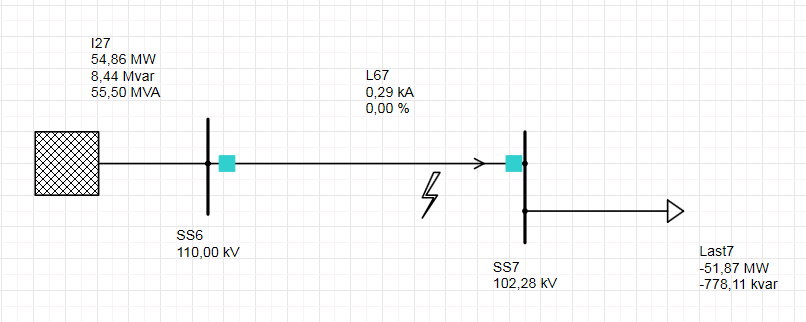
\includegraphics[scale=0.4]{img/distschutz-netz.png}
	\caption{Untersuchtes Netz}
	\end{figure}

	\begin{figure}[H]
	\centering
	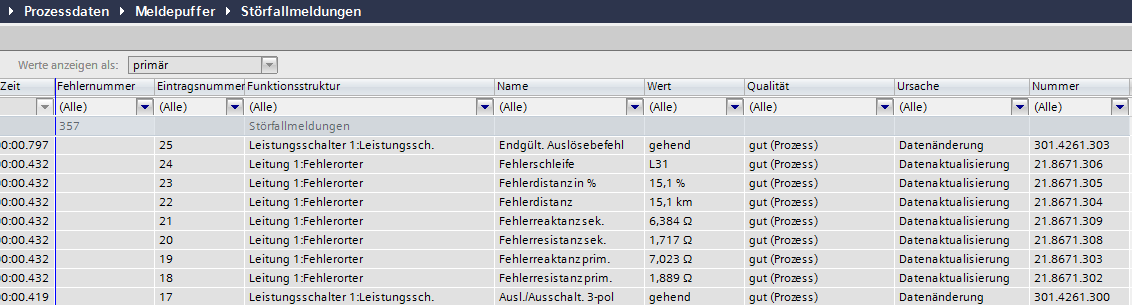
\includegraphics[scale=0.5]{img/digsi.png}
	\caption{Störfallmeldung in DIGSI}
	\end{figure}


\section{Überarbeitung Praktikumversuches}
Der bisher verwendete Praktikumsversuch ist nur teilweise kompatibel mit den Dynamikfunktionen von PSS Sincal. Die Versuchsanleitung muss daher abgeändert. Ein Großteil kann aber aus den ursprünglichen Unterlagen aus Magdeburg weiterverwendet werden.

\subsection{Derzeitige Aufgabenstellung}
Die derzeitige Aufgabenstellung besteht aus fünf Teilen. Zunächst soll das im Vorfeld berechnete Netz in Sincal nachgebaut und ein Kurzschluss auf der Leitung berechnet werden. Die eigenen Rechnungen sollen mit den Werten aus Sincal verglichen werden. \\
Als zweites wird eine dreipolige Kurzschlussstromberechnung an allen Knoten durchgeführt. Es soll dabei einmal der Hochlastfall und einmal der Tieflastfall betrachtet werden. Der Hochlastfall wird dadurch dargestellt, dass die Generatorspannung von G1 auf 105\% bzw. 1,05 p.u. erhöht wird, die Erzeugung der beiden Generatoren beträgt 90\% der Nennleistung mit einem $cos \varphi $ von 0,9. Im Tieflastfall wird G2 vom Netz getrennt, die Spannung von G1 beträgt 100\% bei einer Auslastung von 100\%. Dabei soll an den Knoten $S_k''$, $I_k''$, $I_a$ und $i_p$ aufgenommen werden. \\
Anschließend sollen an insgesamt fünf verschiedenen Punkten Fehleruntersuchungen in verschiedenen Lastfällen durchgeführt werden. Hier soll nur $I_k''$ aufgenommen werden.

\begin{itemize}
\item Hochlastfall Kurzschluss L16 1km Fehlerort A
\item Hochlastfall Kurzschluss L16 49km Fehlerort B
\item Hochlastfall Kurzschluss L67 19km Fehlerort C
\item Hochlastfall Kurzschluss L25 29km Fehlerort D
\item Hochlastfall Kurzschluss L23 44km Fehlerort E
\item Tieflastfall Kurzschluss L23 44km Fehlerort E
\item Tieflastfall Kurzschluss L16 1km Fehlerort A
\end{itemize}

Nach der selben Vorgehensweise werden nun einpolige Erdkurzschlüsse berechnet. Zuerst erfolgt wieder eine gemeinsame Kurzschlussstromberechnung an allen Knoten, anschließend erfolgen die verschiedenen Fehleruntersuchungen. Zuletzt sollen die Ergebnisse diskutiert werden \cite{praktikum-anleitung}.


\subsection{Zukünftige Aufgabenstellung}
An Stelle der Betrachtung der Effektivwerte soll nun in der neuen Aufgabenstellung die Betrachtung der dynamischen Verläufe der Spannungen und Ströme im Vordergrund stehen. Dazu wurden die beiden Aufgabenteile mit den Fehleruntersuchungen angepasst. Die Aufgabenteile mit den Kurzschlussberechnungen an den Sammelschienen wurden komplett übernommen werden. \\
Der erste Aufgabenpunkt, in dem die Studierenden von Hand rechnen und die Ergebnisse mit PSS Sincal vergleichen sollen, muss allerdings abgeändert werden. Da beim Umstellen der verwendeten Lizenz von Sincal die Funktion der Schutzkoordination verloren geht und ein manuelles Umstellen nicht praktikabel ist, soll die Simulation anders durchgeführt werden. Dies geschieht durch Aufteilen der Leitung L23 in zwei Teilstücke und Verbinden dieser mit einem Knoten. Anschließend kann eine dreipolige Kurzschlussberechnung über den Menüpunkt \textit{Berechnen $\rightarrow$ Kurzschluss…} durchgeführt werden. Diese führt an allen Knoten Kurzschlussberechnungen durch, also auch am eingefügten \glqq Fehlerknoten\grqq.

	\begin{figure}[H]
	\centering
	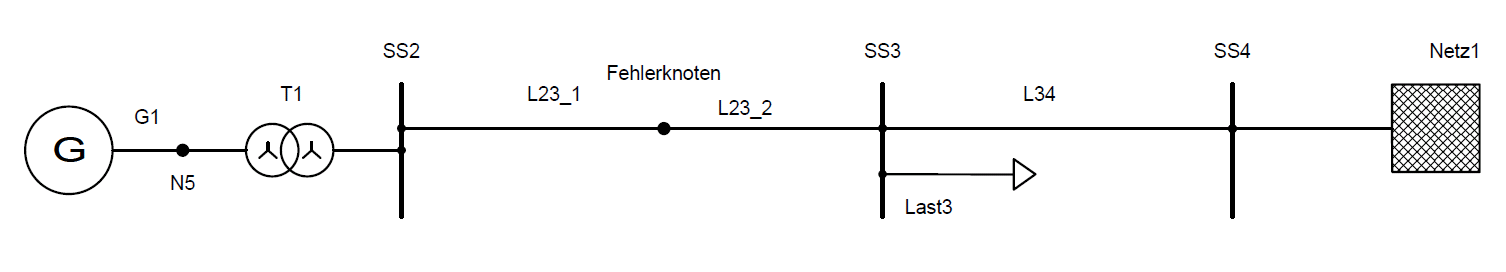
\includegraphics[scale=0.4]{img/ks-versuch_l23.png}
	\caption{Fehlerknoten an L23}
	\label{fehlerknoten_l23}
	\end{figure}

\subsubsection{Festlegen der Plottdefinitionen}
Um die Kurzschlussstromverläufe darzustellen, müssen in Sincal unter dem Punkt Daten $\rightarrow$ Dynamik $\rightarrow$ Plottdefinition… jeweils die aufzuzeichnenden Signale definiert werden. Dabei stellt sich die Frage, an welchen Punkten diese definiert werden, da eine Aufzeichnung des Stromes direkt an der Fehlerstelle nicht möglich ist. Wie in realen Netzen sitzen die Messpunkte jeweils in den Umspannwerken an der Sammelschiene, wodurch bei einem mehrseitig gespeisten Fehler immer nur ein Teilstrom erfasst werden kann. Dies ist, mit Ausnahme von der nur einseitig gespeisten Fehlerstelle C, immer der Fall. Die Messpunkte sollten daher so gewählt werden, dass man \glqq am meisten sieht\grqq:

\begin{itemize}
\item Fehlerstelle A: Spannung: SS1, Strom: SS1 nach L16
\item Fehlerstelle B: Spannung: SS1, Strom: SS1 nach L16
\item Fehlerstelle C: Spannung: SS6, Strom: SS6 nach L67
\item Fehlerstelle D: Spannung: SS5, Strom: SS5 nach L25
\item Fehlerstelle E: Spannung: SS3, Strom: SS3 nach L23
\end{itemize}

Die Messpunkte wurden zum einen so gewählt, dass diese möglichst nahe am Fehlerort liegen (Fehlerorte A, C, D und E) und zum anderen nahe an einem Generator liegen, damit der Abklingvorgang des Kurzschlussstromes sichtbar ist (Fehlerorte A und E). Der Messpunkt für den Fehlerort B wurde ebenfalls auf die Sammelschiene SS1 gelegt, um den Einfluss der Leitungsimpedanz zwischen Fehlerort A und B zu verdeutlichen. \\
Die Spannung soll als Leiter-Erdspannung gemessen werden, damit insbesondere beim einpoligen Erdkurzschluss die Spannungserhöhung der fehlerfreien Leiter sichtbar wird. \\
In den Berechnungsparametern sollten zudem für die Aufgabenstellung sinnvolle Zeiteinstellungen vorgenommen werden. Eine Endzeitpunkt von 0,5s und ein Zeitschritt von 0,001s erwiesen sich als sinnvoll.
%\\ Lösung und Anleitung dann noch falsch (Fehlerort B)!!!


\subsubsection{Fehlerbedingungen}
Der Aufgabenteil \glqq Variation des Kurzschlussortes bei einem dreipoligen Fehler\grqq{} kann ebenfalls komplett übernommen werden. Mit der dynamischen Betrachtung der Kurzschlussströme lassen sich nun aber auch die anderen Untersuchungen aus den Praktikumsunterlagen aus Magdeburg durchführen. Diese beinhalten die Betrachtungen bei unterschiedlichen Fehlereinschaltzeiten, Kurzunterbrechungen und einpolige Fehler. Diese sind:

\begin{itemize}
\item Kurzschlusseintritt bei Spannungsmaximum
\item Kurzschlusseintritt bei Spannungsnulldurchgang
\item Kurzschlusseintritt bei U = 0.5 p.u.
\item Kurzschlussabschaltung nach 120ms
\item Kurzschlussabschaltung nach 120ms mit Kurzunterbrechung (100ms) (AWE mit Erfolg)
\item Kurzunterbrechung nach 100ms ohne Kurzschlussabschaltung (AWE ohne Erfolg)
\item Erdkurzschluss AWE mit Erfolg
\item Erdkurzschluss AWE ohne Erfolg
\end{itemize}

Alle Fehleruntersuchungen können mit Hilfe der Dynamikberechnungen von PSS Sincal durchgeführt werden. Allerdings sind in den Praktikumsunterlagen aus Magdeburg für diese Fehleruntersuchungen keine Fehlerorte gegeben. Der Einfachheit wegen und besseren Vergleichbarkeit der Lösungen sollen diese nun für Bielefeld vorgegeben werden. Dafür wurde der Fehlerort A ausgewählt (warum?). Für jede Fehleruntersuchung soll von allen Phasen jeweils der Strom aufgenommen werden, für die Fehleruntersuchungen mit Kurzschlussabschaltung oder Kurzunterbrechung auch die Spannung.

Für die insgesamt vier Fehleruntersuchungen mit AWE müssen Elementschaltzeiten mit einbezogen werden. Diese sind in den Abbildungen \ref{awe-me} und \ref{awe-oe} dargestellt. Der Fehler tritt zum Zeitpunkt Null auf. 100ms nach Fehlereintritt löst der Schutz zum ersten mal aus und schaltet den Fehler ab. Geschieht dies von zwei Seiten, so müssen die Elementschaltzeiten unterschiedlich sein, da Sincal ansonsten die Berechnung mit einem Fehler abbricht. So kann eine Seite bei 100ms abgeschaltet werden, die andere bei 101ms.

Insgesamt

	\begin{figure}[H]
	\centering
	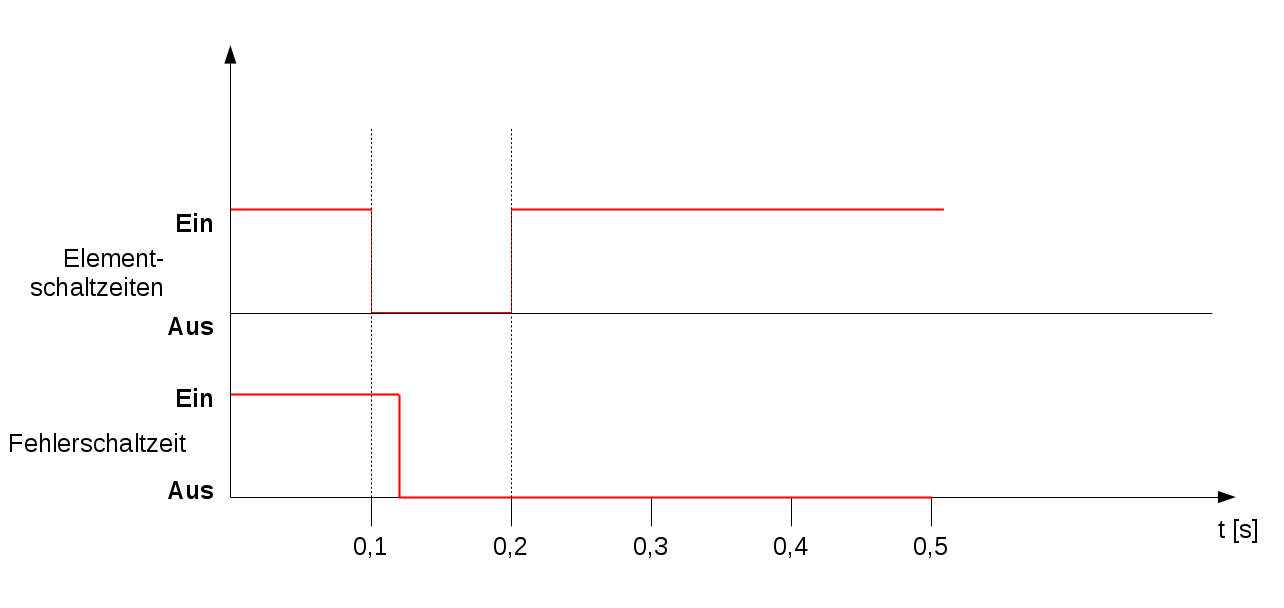
\includegraphics[scale=0.45]{img/awe-me.png}
	\caption{AWE mit Erfolg}
	\label{awe-me}
	\end{figure}

	\begin{figure}[H]
	\centering
	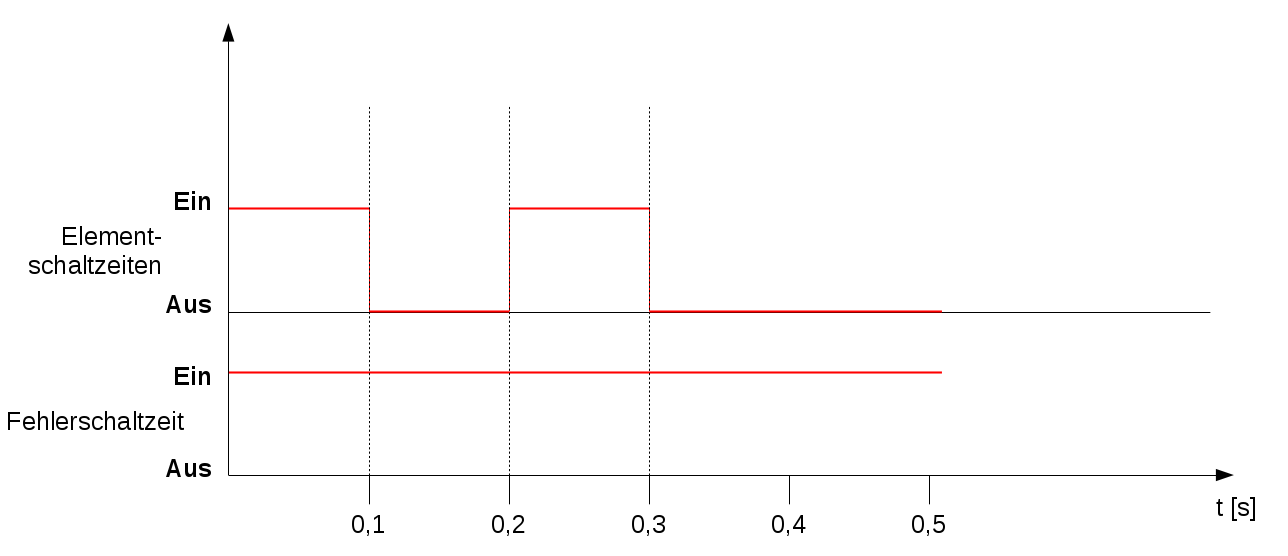
\includegraphics[scale=0.45]{img/awe-oe.png}
	\caption{AWE ohne Erfolg}
	\label{awe-oe}
	\end{figure}


Bei den beiden letzten Berechnungen, die eine einpolige AWE beinhalten, traten Probleme auf, die nicht direkt lösbar waren. Zunächst wurde die Fehleruntersuchung zu einem einpoligen Erdkurzschluss auf L1 geändert, anschließend die Elementschaltzeiten so, dass diese nur L1 schalten sollen. Sincal beendete darauf hin die Berechnungen, da anscheinend für solche Berechnungen keine Lizenz vorliegt. Das Lizenzproblem liegt anscheinend an den Elementschaltzeiten, da ein Berechnen von einpoligen Fehlern bei dreipoligen Elementschaltzeiten möglich ist.

	\begin{figure}[H]
	\centering
	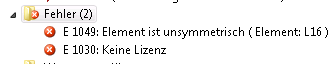
\includegraphics[scale=1]{img/keine-lizenz.png}
	\caption{Lizenzfehlermeldung}
	\label{awe-oe}
	\end{figure}

Daher sollen im Praktikumsversuch die Erdkurzschlüsse ebenfalls mit einer dreipoligen Kurzunterbrechung simuliert werden, auch wenn dies nicht unbedingt der Realität in Europa entspricht.


\subsubsection{Anleitung und Musterlösungen}
Um die Studierenden besser zu unterstützen, wurden für die Praktikumsanleitung Hinweise ausgearbeitet, die den Umgang mit PSS Sincal vereinfachen sollen. Dort ist unter anderem mit Screenshots erkärt, wie Fehleruntersuchungen eingefügt und Signale in Diagrammen grafisch dargestellt werden können. Diese Hinweise finden sich im Anhang der überarbeiteten Praktikumsanleitung.\\
Des weiteren wurden für sämtliche Fehleruntersuchungen Musterlösungen in Form von Screenshots erstellt.

\subsection{Probleme bei der Umsetzung des Versuches}
Die Tatsache, dass im Gegensatz zu den EduTrans-Lizenzen mit 25 gleichzeitigen Benutzern nur sechs gleichzeitige Benutzer erlaubt sind, kann in der Praxis zu Problemen führen. Im Labor F103 \glqq elektrische Netze\grqq{} befinden sich derzeit acht PCs, es sind also zwei Lizenzen zu wenig vorhanden. Als Abhilfe könnten die anderen beiden Rechner jeweils eine EleKey2-Lizenz verwenden, die ebenfalls die Berechnung von elektromagnetischen Transienten erlaubt. Somit könnte wie gewohnt an allen acht Rechnern gleichzeitig gearbeitet werden.

\section{Zusammenfassung}

\newpage
\pagenumbering{Roman}
\setcounter{page}{1}
\section{Literaturverzeichnis}
Hinweis: \cite{hybrid-ltg} und \cite{phasenschieber-biblis} konnten Online nicht mehr aufgefunden werden, daher liegen diese beiden Präsentationen der CD als PDF bei.

\bibliography{bibtest1}
\bibliographystyle{unsrtdin}

\section{Anhang}
\subsection{Netz Laborversuch}
\begin{table}[H]
\begin{tabular}{|c|c|}
\hline 
\textbf{Bezeichnung} & \textbf{Netz 1} \\ 
\hline 
Kurzschlussleistung $S_k''$ & 1000MVA \\ 
\hline 
Kurzschlussleistung $S_k''$ Maximum & 1000 \\ 
\hline 
Kurzschlussleistung $S_k''$ Minimum & 1000 \\ 
\hline 
Verhältnis R/X & 0.1 p.u. \\ 
\hline
\end{tabular} 
\caption{Nenndaten des starren Netzes}
\end{table}

\begin{table}[H]
\begin{tabular}{|c|c|c|}
\hline 
\textbf{Bezeichnung} & \textbf{Transformator 1} & \textbf{Transformator 2} \\ 
\hline 
Nennspannung Seite 1 $U_{n1}$ & 110kV & 110kV \\ 
\hline 
Nennspannung Seite 2 $U_{n2}$ & 10kV & 10kV \\ 
\hline 
Nennscheinleistung $S_n$ & 100MVA & 80MVA \\ 
\hline 
Dauerleistung $S_{max}$ & 100MVA & 80MVA \\ 
\hline 
Kurzschlussspannung $u_k$ & 12\% & 12\% \\ 
\hline 
Ohmsche Kurzschlussspannung $u_r$ & 0,38\% & 0,38\% \\ 
\hline 
Schaltgruppe & Yy0 & Yy0 \\ 
\hline 
\end{tabular}
\caption{Nenndaten Transformatoren}
\end{table}

\begin{table}[H]
\begin{tabular}{ll}

\begin{tabular}{|c|c|}
\hline 
\textbf{Bezeichnung} & \textbf{Kenndaten} \\ 
\hline 
Leitungstyp & Freileitung \\ 
\hline 
Widerstand r & 0,118 Ohm/km \\ 
\hline 
Reaktanz x & 0,421 Ohm/km \\ 
\hline 
Kapazität c & 9,17nF/km \\ 
\hline 
Nennspannung & 110kV \\ 
\hline 
Therm. Grenzstrom & 645A \\ 
\hline 
\end{tabular}

&

\begin{tabular}{|c|c|}
\hline 
\textbf{Leitung} & \textbf{Länge} \\ 
\hline 
L12 & 30km \\ 
\hline 
L16 & 50km \\ 
\hline 
L23 & 45km \\ 
\hline 
L25 & 30km \\ 
\hline 
L34 & 25km \\ 
\hline 
L45 & 20km \\ 
\hline 
L64 & 35km \\ 
\hline 
L67 & 20km \\ 
\hline 
\end{tabular}

\end{tabular}

\caption{Freileitungen}
\end{table}

\begin{table}[H]
\begin{tabular}{|c|c|c|}
\hline 
\textbf{Last} & \textbf{Scheinleistung} & \textbf{Leistungsfaktor} \\ 
\hline 
Last 1 & 40MVA & 0,95 \\ 
\hline 
Last 2 & 30MVA & 0,8 \\ 
\hline 
Last 3 & 60MVA & 0,9 \\ 
\hline 
Last 5 & 40MVA & 0,9 \\ 
\hline 
Last 7 & 60MVA & 0,9 \\ 
\hline 
\end{tabular}
\caption{Lasten}
\end{table}

\begin{table}[H]

\begin{tabular}{|l|c|c|}
\hline 
\textbf{Bezeichnung} & \textbf{Generator 1} & \textbf{Generator 2} \\ 
\hline 
Maschinentyp & Turbogenerator & Turbogenerator \\ 
\hline 
Bemessungsscheinleistung & 100MVA & 80MVA \\ 
\hline 
Bemessungsspannung & 10kV & 10kV \\ 
\hline 
Verhältnis R/X & 0,1 p.u. & 0,1 p.u. \\ 
\hline 
Anlaufzeitkonstante $T_A$ & 8,2s & 8,2s \\
\hline
Gleichstromzeitkonstante $T_G$ & 0,36s & 0,36s \\
\hline
Ankerwiderstand $R_a$ & 0,01 p.u. & 0,01 p.u. \\
\hline
Ankerstreureaktanz $X_{1\sigma}$ & 0,13 p.u. & 0,13 p.u. \\
\hline
\multicolumn{3}{|l|}{Kurzschlusszeitkonstanten} \\
\hline
• subtransient d-Achse $T_d''$ & 0,03s & 0,03s \\
\hline
• subtransient q-Achse $T_q''$ & 0,03s & 0,03s \\
\hline
• transient d-Achse $T_d'$ & 1,0s & 1,0s \\
\hline
• subtransient q-Achse $T_q'$ & 1,0s & 1,0s \\
\hline
\multicolumn{3}{|l|}{Reaktanzen} \\
\hline
• subtransient d-Achse $X_{d}''$ & 20\% & 20\% \\ 
\hline
• subtransient q-Achse $X_q''$ & 20\% & 20\% \\
\hline
• transient d-Achse $X_{d}''$ & 30,1\% & 30,1\% \\ 
\hline
• transient q-Achse $X_q''$ & 100\% & 100\% \\
\hline
• stationär d-Achse $X_d$ & 227\% & 227\% \\
\hline
• stationär q-Achse $X_q$ & 205\% & 205\% \\
\hline
Bemessungsleistungsfaktor & 0,9 & 0,9 \\ 
\hline 
Wirkleistung P & 90MW & 72MW \\ 
\hline 
Generatorspannung & 10kV & 10kV \\ 
\hline
\end{tabular}

\caption{Generatoren}
\end{table}


	\begin{figure}[H]
	\centering
	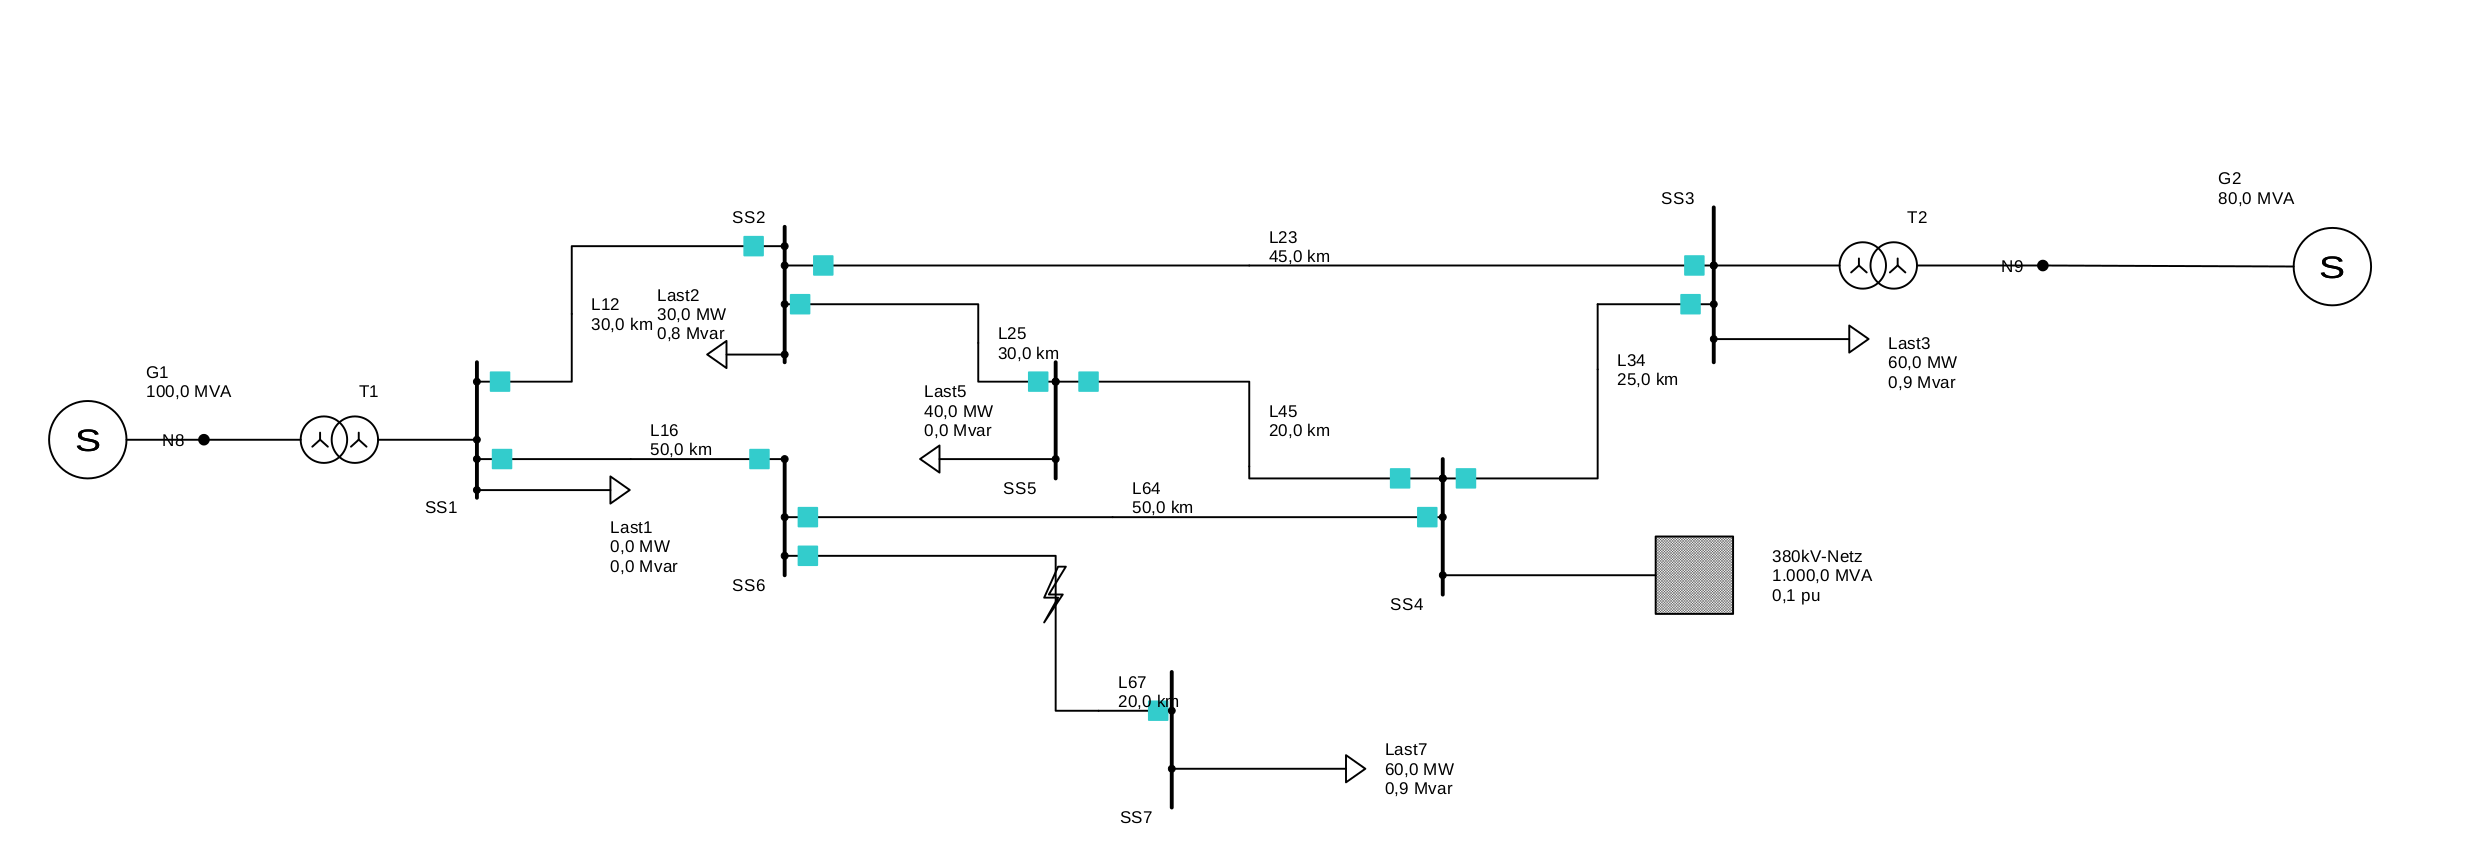
\includegraphics[scale=0.35, angle=90]{img/praktikum-netz}
	\caption{Netzaufbau Laborversuch}
	\label{praktikum-netz}
	\end{figure}
	
\subsubsection*{Dateien auf DVD}
\begin{itemize}
\item Bachelorarbeit.pdf
\item comtrade-adjust.vbscript
\item Sincal-Projekt Kurzschlussversuch
\item Überarbeiteter Laborversuch
\end{itemize}

\end{onehalfspace}

\end{document}

